\def\documentclassname{ctexart}
\documentclass[a4paper]{\documentclassname}
\usepackage{amsmath}
\usepackage{amssymb}
\usepackage{amsthm}
%\usepackage{color}
\usepackage{graphicx}
%\usepackage{geometry}
\usepackage{hyperref}
\usepackage{ifthen}
%\usepackage{marginnote}
%\usepackage{mathrsfs}
%\usepackage{syntonly}
%\usepackage{textcomp}
\usepackage{ulem}
%\usepackage{verbatim}
%\syntaxonly
%\geometry{a5paper}
\hyphenation{}
\normalem
\hypersetup{
    colorlinks,
    linkcolor=blue,
    citecolor=red,
    filecolor=cyan,
    urlcolor=magenta,
}
\allowdisplaybreaks
\def\b{\boldsymbol}
\def\d{\mathrm{d}}
\def\f{\frac}
\def\p{\partial}
\def\ph{\phantom}
\def\t{\text}
\def\ti{\tilde}
\def\v{\vec}
\def\La{\Leftarrow}
\def\Ra{\Rightarrow}
\newcommand{\tabincell}[2]{\begin{tabular}{@{}#1@{}}#2\end{tabular}}
\DeclareMathOperator{\atanxy}{atan2}
\DeclareMathOperator{\sinc}{sinc}
\DeclareMathOperator{\sgn}{sgn}
\DeclareMathOperator{\Arg}{Arg}
\theoremstyle{definition}
\ifthenelse{\equal{\documentclassname}{article}}{
    \newtheorem{definition}{Definition}
    \newtheorem{theorem}{Theorem}
}{}
\ifthenelse{\equal{\documentclassname}{ctexart}}{
    \newtheorem{definition}{定义}
    \newtheorem{theorem}{定理}
}{}
\title{LIGO-Virgo探测器噪声和瞬变引力波信号的提取的指南}
\author{LIGO科学合作组织和Virgo合作组织}
\date{}
\begin{document}

\maketitle

\begin{abstract}
    LIGO科学合作组织和Virgo合作组织在先进探测器时代的前两次观测中, 已经对11个被可靠探测到的引力波事件进行了编目. 所有11个事件都与紧凑的恒星质量天体 (黑洞或中子星) 之间的良好建模并合一致. 这些事件中的每一个时间的数据都已通过引力波开放科学中心公开提供. 第一次和第二次观测运行的全部引力波应变数据现在也已公开. 广泛的科学界对理解分析中使用的数据和方法有着相当大的兴趣. 在本文中, 我们概述了探测器噪声特性以及用于观测引力波信号和推断源特性的数据分析技术. 我们描述了一些为验证引力波事件观测的分析和结果而执行的检查. 我们还解决了人们对LIGO-Virgo探测器噪声的各种特性以及应用于结果数据的分析的正确性的担忧. 
\end{abstract}

\section{引言}

引力波观测已成为了解宇宙的重要新手段. LIGO科学合作组织和Virgo合作组织(LVC)发表了一系列发现, 从第一个探测到的事件GW150914[1]开始, 这是一个双黑洞并合. 在两年的时间里, 该事件之后又进行了9次双星探测 (GW151012 [2,3], GW151226[4], GW170104[5], GW170608[6], GW170729, GW170809, GW170814[7], GW170818和GW170823) , 以及一次双中子星并合, GW170817 [8]. 关于所有这些被可靠探测到的引力波事件的细节已经发表在一个目录中, GWTC-1[3]. 

全球引力波探测器网络目前由美国Washington州Hanford和Louisiana州Livingston的两个先进LIGO探测器[9]组成;意大利Cascina的Advanced Virgo探测器[10];以及德国的GEO 600探测器[11]. 在未来几年中, 该网络将通过增加日本探测器KAGRA [12-14]和位于印度的第三个Advanced LIGO探测器[15]来发展. Advanced LIGO的第一次观测运行 (O1) 于2015年9月12日至2016年1月19日进行. Advanced LIGO探测器的第二次观测运行 (O2) 于2016年11月30日开始, 一直持续到2017年8月25日. Advanced Virgo探测器于2017年8月1日正式开始在O2中观测, 实现了首次三探测器对引力波的观测[3]. 2019年4月1日, LIGO-Virgo的第三次观测运行O3开始, 所有三个探测器都以迄今为止最好的灵敏度运行. 

多个探测器之间的一致性极大地有助于抑制仪器背景, 并允许对引力波信号进行相干分析. 迄今为止公布的所有事件探测都涉及Advanced LIGO探测器, 而GW170814和GW170818也是Virgo感应的三重探测. Virgo的数据也被用于GW170729, GW170809和GW170817的参数估计分析和天空定位确定. Virgo的数据在帮助找到GW170817的来源方面尤为关键[16]. 这次双中子星并合代表了多信使天文学与引力波的非凡首次亮相, 因为它紧随其后的是短伽马射线暴GRB 170817A [17,  18], 从引力波数据中获得的相对精确的定位使得能够识别和深入研究来自光学对应物SSS17a / AT 2017gfo的千新星和余辉发射[16,  19]. 

如[3]所述, LVC观测是使用两个独立的匹配滤波器分析进行的, 用于搜索O2中的紧凑双星聚结[20,21], 以及用于短期瞬态信号或突发的未建模搜索[22]. 因此, 由LVC开发并使用添加到模拟数据中的模拟信号进行测试的观测方法, 或者添加到先前的真实数据集中, 其中任何可能的信号都被噪声淹没, 现在已经被证明对天体物理引力波信号是有效的. LVC分析的测试和验证是通过在分析中执行的 (模拟) 信号注入 (即在软件中) 和在硬件中通过移动探测器的测试质量进行的信号注入来实现的. 

观测到的引力波事件数量的增加激发了人们对探测源的天体物理学影响的浓厚兴趣, 以及对引力波数据的兴趣. 目前, LVC通过引力波开放科学中心 (GWOSC) 发布数据[23,24]. LIGO数据发布在LIGO数据管理计划[25]中有所描述, 该计划是LIGO实验室与美国国家科学基金会之间的一项协议. [26,  27]介绍了释放引力波触发器和候选事件的LVC策略. 对于紧凑二元并合的观测, 在发布时会发布事件时间前后约一小时 ($4096\t{s}$) 的标定应变数据. 这些数据可用于O1和O2中所有已发表的观测结果[28]. 

目前, GWOSC上提供了自2005年以来首次LIGO科学运行的大量数据[24], O1观测运行的Advanced LIGO数据[29]以及O2观测运行的Advanced LIGO和Advanced Virgo数据[30]. 数据管理计划中描述了未来观测运行中数据发布的时间[25];例如, O3 运行前 6 个月的批量数据将于 2021 年 4 月发布. GWOSC不断更新和发布数据产品, 以满足更广泛的科学界的需求和利益. 合作使用的许多分析软件包都以开源代码的形式公开提供;GWOSC网站[24]上提供了这些清单. 此外, 通过LIGO文件控制中心发布了一些中间数据产品, 这些产品通常与LVC论文相关联;例如, 参见[31]. 

随着LIGO和Virgo数据的公开发布, 这些合作之外的团队正在分析发布的数据. 这些分析中的大多数得出的结果与LVC一致[32-39], 并且还报道了一些其他重要候选事件[40,41].  LIGO数据的噪声特性和GW150914的LVC数据分析的正确性也受到质疑[42,43], 尽管连续的引力波探测增强了我们的探测和参数估计方法的信心[3]. 出于对分析LIGO和Virgo数据的广泛兴趣, 本文概述了LIGO-Virgo数据的特性及其噪声分量. 我们还描述了数据分析程序的基本特征, 这些程序已被LIGO和Virgo团队用于观测和测量编目的引力波源的特性[3], 如图1所示. 在寻找引力波信号时, 对LIGO和Virgo数据的分析是复杂的, 正确处理噪声的统计特性也是如此. LVC鼓励更广泛的科学界访问和分析其数据, 并将始终对有关其用来得出结论的方法的讨论持开放态度. 用于分析LIGO-Virgo数据的代码是公开的. 本文中用于生成许多数字的特殊用途代码也可用[44]. 此外, LVC还提供了一个Jupyter笔记本, 以简化的实现方式说明用于生成关键指标和结果的方法[45]. 最后, LVC用于处理LIGO-Virgo数据, 搜索事件和表征观测信号的许多软件包都可以在GWOSC站点找到[46]. 
\begin{figure}[htbp]
    \centering
    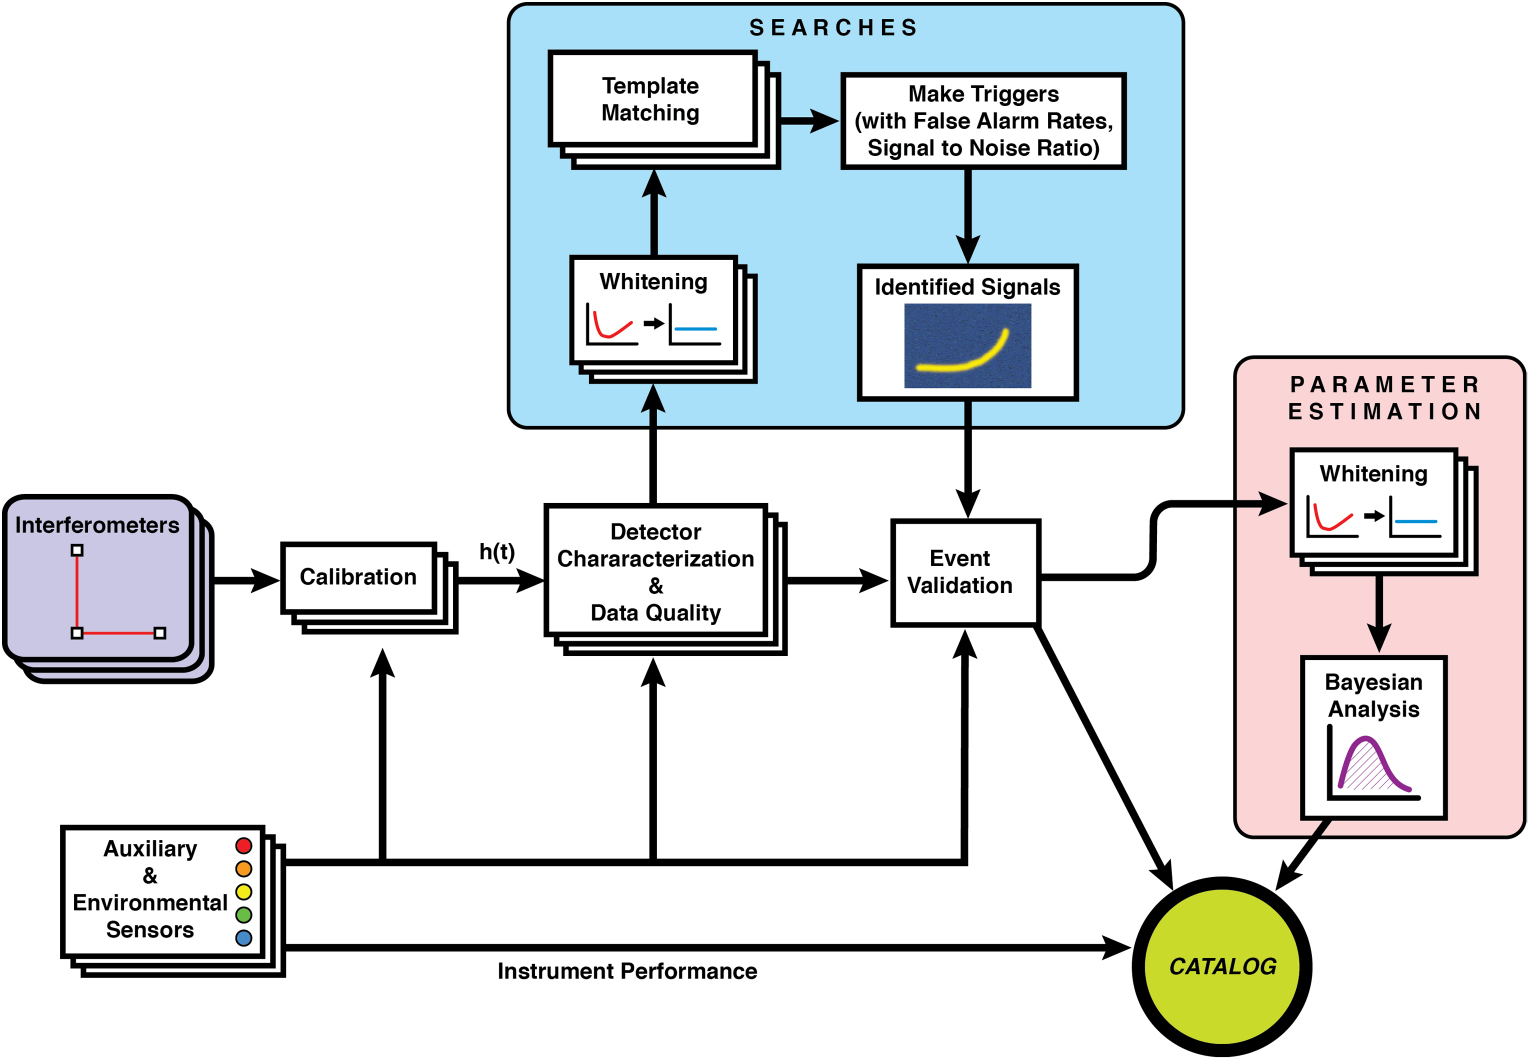
\includegraphics{img/1.jpg}
    \caption{
        一个简化的原理图, 总结了LIGO-Virgo数据处理的主要步骤, 从数据输出到瞬态事件目录中报告的结果. 
    }
\end{figure}

本文组织如下. 在第2节中, 我们描述了LIGO-Virgo数据的属性, 而在第3节中, 我们将讨论影响这些数据的噪声. 第 4 节介绍了用于正确Fourier 变换数据和估计功率谱的基本数据处理步骤. 第5节介绍了基于小波的时频方法, 可用于评估与稳态检波器噪声的可能偏差. 第6节讨论了LIGO和Virgo的探测器和标定问题. 第 7 节介绍了用于定义参数估计研究中使用的似然函数的噪声模型. 第 8 节描述了 LVC 搜索引力波信号的方法, 而第 9 节介绍了 LVC 推断观测到的波形并估计发射引力波的系统的物理参数的方法. 为了说明这些概念, 第10节简要介绍了如何使用公开发布的GW150914数据来查找最佳拟合波形模型并研究残差的相关性. 我们还讨论了[42,43]中关于探测器噪声, 残差和GW150914源属性估计相关性的声明. 在解决这些说法时, LVC指出, 参与我们合作的外部团体可以引入新的想法和技术, 这对引力波科学是有益的. 最后, 在第11节中, 我们对LIGO和Virgo数据属性进行了总结评估, 并提供了LVC数据分析结果和验证. 

\section{LIGO-Virgo数据的性质}

Advanced LIGO [9] 和 Advanced Virgo [10] 第二代引力波探测器是大规模增强型Michelson干涉仪. 探测器对通过引力波引起的时空应变以及等效的与地球有关的力和位移噪声很敏感, 每一种噪声都会导致臂的长度随时间变化. 相对臂长度的差异会在增强型Michelson输出中产生功率变化, 并由光电二极管捕获. 来自这些光电二极管的信号既用作引力波读数, 也用作控制大约100 Hz以下的相对臂长度的误差信号. 

Advanced LIGO引力波探测器在设计上是相同的, 都有$4\t{km}$长的臂. Advanced Virgo也有类似的设计, 手臂长$3\t{km}$. Fabry-Perot腔用于探测器的臂中, 以增加与引力波的相互作用时间, 并使用功率回收来增加有效激光功率. Advanced LIGO探测器中增加了信号回收函数, 以形成其频率响应[9]. Advanced Virgo尚未实现信号回收, 但将来会[10]. 

对每个探测器的干涉仪光电二极管输出 (见第6.1节) 应用标定程序, 以产生作为时间序列的引力波应变数据, LIGO数据的采样率为$16384 \t{Hz}$, Virgo数据的采样率为$20 \t{kHz}$. 对于Advanced LIGO探测器, 标定在$10 \t{Hz}$以上和$5 \t{kHz}$以下有效, 如第6.1节所述. 对于O2中的Advanced Virgo, 标定有效性范围为$10 \t{Hz}$至$8 \t{kHz}$ [47]. 探测器还记录数十万个辅助通道, 除了应变信号外, 还记录时间序列, 用于监控探测器的行为及其环境. GWOSC 提供了经过提炼的额外数据通道, 在这些通道中, 实施了与数据质量不同级别的问题相关的标志\footnote{\href{www.gw-openscience.org/segments}{www.gw-openscience.org/segments}}.我们采用对探测器性能的连续监测来表征可能对搜索灵敏度或源属性估计产生负面影响的噪声源[48,49].  如第6节和[50]所述, 由于探测器故障, 标定错误或数据采集问题导致的无效数据将被标记, 以便从分析中删除它们. 

\section{探测器噪声的基本特性}

Advanced LIGO和Advanced Virgo仪器记录的数据受到许多噪声源的影响, 包括量子传感噪声, 地震噪声, 悬浮热噪声, 镜面涂层热噪声和重力梯度噪声[9]. 此外, 还有瞬态噪声事件, 例如来自人为来源, 天气, 设备故障[48], 以及偶尔出现的不明来源的瞬态噪声[51]. 此外, 还存在持续升高的噪声, 仅限于某些频率, 在噪声与频率的关系图中表现为非常窄的峰值, 我们称之为频谱线; 这些通常是由电气和机械设备或共振引起的[49]. 检波器中所有噪声源的组合产生一个时间序列$n(t)$, 可以用向量$\b{n}$表示, 其分量由离散时间样本$n_i=n(t_i)$给出. 噪声被描述为一个随机过程, 其统计属性由联合概率分布$p(\b{n})$给出. 此模型可用于定义汇总统计量, 例如平均值$\b{\mu}=\mathrm{E}(\b{n})$ (其中$\mathrm{E}$定义为期望值) 和协方差$C_{ij}=\mathrm{E}[(n_i-\b{\mu})(n_j-\b{\mu})]$其中期望值是相对于$p(\b{n})$.从数据中可以估计出平均值为
\begin{equation}
    \hat{\b{\mu}}=\frac{1}{N}\sum_{i=1}^N n_i,
\end{equation}
其中$N=\mathrm{dim}(\b{n})$是数据样本的数量. 如果不做出额外的假设, 就无法从数据中估计完整的协方差矩阵, 因为我们每个数据点只有$ M = 1 $个测量值, 这使得样本协方差矩阵在形式上未定义:
\begin{equation}
    \hat{C_{ij}}=\frac{1}{M-1}(n_i-\hat{\b{\mu}})(n_j-\hat{\b{\mu}}).
\end{equation}
如果假设噪声遵循特定分布, 或者噪声属性在时间上保持不变, 则可以对协方差矩阵进行估计. 请注意, 在实践中, 分析通常不会一次使用所有$ N $个样本, 而是使用不同长度的连续数据片段, 从几秒钟到几小时不等, 具体取决于预期应用. 如果联合概率分布服从多元正态分布, 则噪声称为Gaussian 分布:
\begin{equation}
    p(\b{n})=\frac{1}{\mathrm{det}(2\pi\b{C})^{1/2}}\exp\left[-\frac{1}{2}\sum_{ij}(n_i-\b{\mu})(n_j-\b{\mu})C_{ij}^{-1}\right],
\end{equation}
 
其中$C_{ij}^{-1}$是协方差矩阵的逆. 如果 $C_{ij}$仅取决于间隔$|i-j|$则噪声被称为稳态的. 稳态噪声被相关函数$C(\tau)$表征, 其中$\tau|t_i-t_j|$是时间间隔. 转换为Fourier域, 其中标签$i$, $j$现在指频率$f_i$, $f_j$, 稳态噪声具有对角协方差矩阵$C_{ij}=\delta_{ij}S_n(f_i)$, 这定义了功率谱密度$S_n(f)$. 功率谱密度由相关函数$C(\tau)$的Fourier变换给出. 振幅谱密度是功率谱密度的平方根, 单位为 $\t{Hz}^{-1/2}$. 如果在频域和时域中都有$C_{ij}=\delta_{ij}\sigma^2$则噪声称为白的. 然而, 白噪声是LIGO-Virgo探测器噪声的粗劣近似.

了解噪声对于探测引力波信号和推断产生引力波信号的天体物理源的特性至关重要. 如果对噪声建模不当, 可能会导致事件的重要性被错误估计, 并导致参数估计中出现系统性偏差. 为了防止这些不良结果, 探测器表征和噪声建模是LVC中的重要活动[48,50].  虽然许多教科书上对引力波数据分析的处理[52-54]描述了独立探测器具有稳态Gaussian噪声的理想化情况, 但实际的LVC分析却小心翼翼地解释了与这一理想的偏差. 

Advanced LIGO和Advanced Virgo探测器数据在时间和频率上都具有丰富的结构. 对于给定的引力波源, 噪声 (由其频谱密度描述) 决定了测得的信噪比 (SNR) . 图2显示了LIGO-Livingston探测器在首次探测到双中子星并合引力波, GW170817, 前三分钟内的平均光谱频率含量. 在O1和O2运行期间, AdvancedLIGO探测器的平均测量噪声幅度约为$10^{-23}\t{Hz}^{-1/2}$在$100 \t{Hz}$时 (Advanced LIGO在$100 \t{Hz}$时的目标灵敏度为$\t{Hz}^{-1/2}$ [9], 而对于Advanced Virgo来说, 它是$\t{Hz}^{-1/2}$ [10].)  低频时的陡峭形状以与地面运动相关的噪声为主. 在大约 $100\t{Hz}$以上, Advanced LIGO探测器目前受到量子噪声限制, 其噪声曲线以散粒噪声为主[9,55]. 在某些频率下, 数据中也存在高振幅噪声特征, 包括由交流电网引起的线路 (美国为  $60\t{Hz}$, 欧洲为  $50\t{Hz}$) , 镜子悬浮液的机械共振, 注入的标定线路以及通过探测器控制系统进入的噪声. 有关Advanced LIGO探测器中在特定频率出现的噪声源的详细说明, 请参见[49]. 有关用于观测运行O2的Advanced Virgo噪声线的列表, 请参见[56]. 
\begin{figure}[htbp]
    \centering
    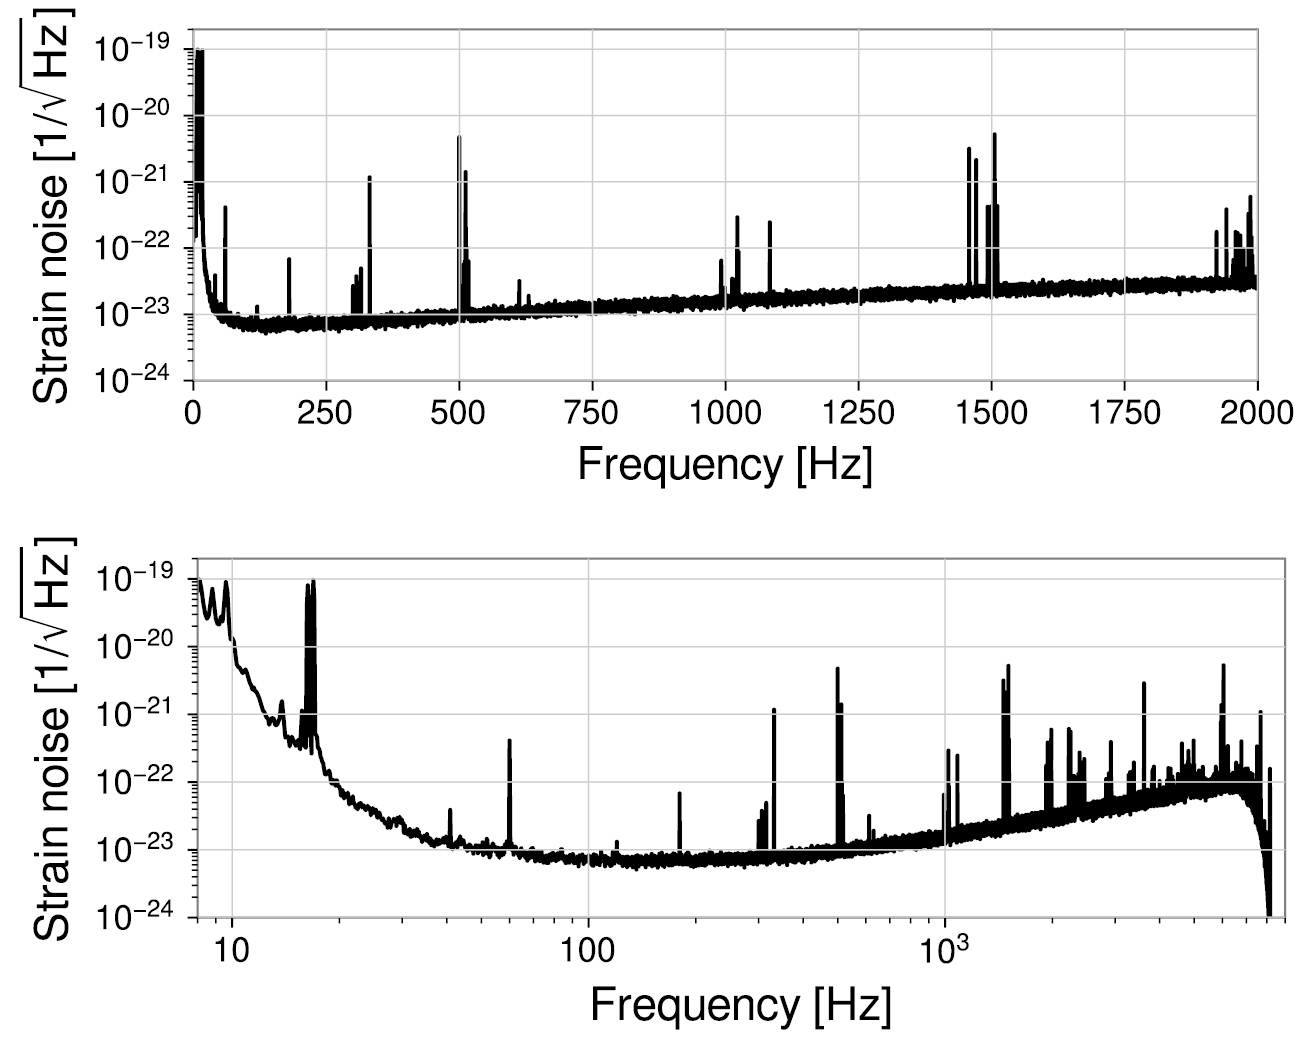
\includegraphics{img/2.jpg}
    \caption{
        LIGO-Livingston探测器数据的振幅光谱密度, 使用 $10\t{s}$快速Fourier变换, 从2017年8月17日12:36:00 UTC开始的三分钟内取平均值, 比GW170817并合时间早5分钟[8]. 顶部图是线性频率刻度, 突出显示了  $0\t{Hz}$ 至  $2000\t{Hz}$ 的周期性特征. 下图是对数刻度, 表示从 $8\t{Hz}$到Nyquist 频率 $8192\t{Hz}$的检波器数据中的特征. 
    }
\end{figure}

\section{Fourier域分析}

LIGO-Virgo探测器中的噪声除了个别例外外, 几乎是稳态的, 因此在频域中最容易表征. 稳态Gaussian 噪声在频率统计堆栈之间不相关, 在每个统计堆栈中的噪声$\ti{n}(f)$都遵循具有随机相位和振幅$S_n^{1/2}(f)$的Gaussian 分布. 许多LVC分析的第一步是使用快速Fourier变换 (FFT) 对时域数据进行Fourier变换[57-59]. 由于FFT隐含地假设被转换的数据在时间上是周期性的, 因此必须将窗函数[60,61]应用于数据, 以抑制频谱泄漏[61], 例如使用Tukey (余弦锥形) 窗函数. 如果不能对数据进行窗化处理, 将导致频谱泄漏和统计堆栈之间相位的虚假相关性. 对于瞬态数据的分析, 使用Tukey窗是有利的, 因为信号比Hanning或Flattop窗受到的修改更少[61]. 

举例来说, 图3显示了在GW150914前后, LIGO-Hanford探测器对一段标定的应变数据应用的一系列处理步骤. 原始数据以低频噪声为主. 对原始数据应用了具有 $0.5 \t{s}$ 过渡区域的 Tukey 窗. 接下来, 通过将Fourier系数除以噪声振幅谱密度的估计值来对数据进行白化(whiten), 这通过对噪声较大的频率进行减权, 从而确保每个频率统计堆栈中的数据具有相等的显著性. 然后对数据进行逆Fourier变换以返回到时域:
\begin{equation}
    d(t)\xrightarrow[]{\text{FFT}}\ti{d}(f)\xrightarrow[]{\text{Whiten}}\ti{d}_w(f)=\frac{\ti{d}(f)}{S_n^{1/2}(f)}\xrightarrow[]{\text{iFFT}}d_w(t).
\end{equation}
\begin{figure}[htbp]
    \centering
    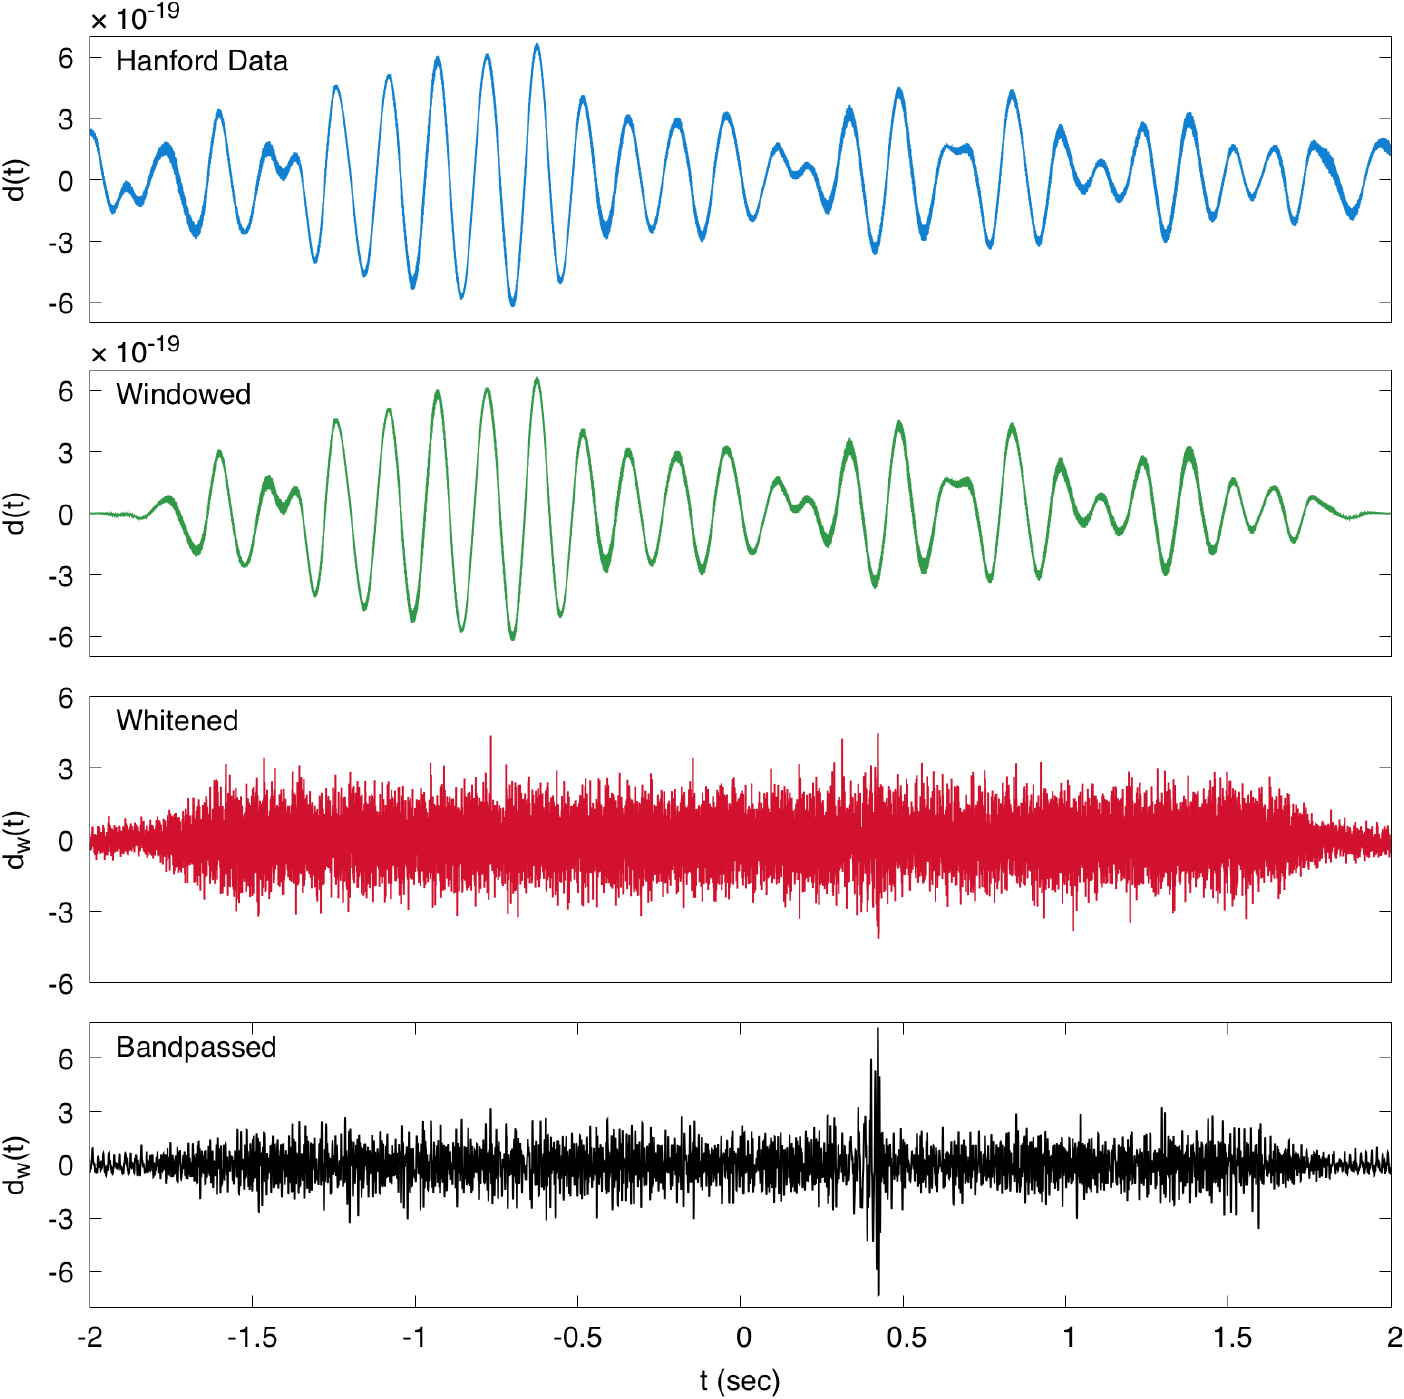
\includegraphics{img/3.jpg}
    \caption{
        应用于LIGO-Hanford探测器标定应变的一系列处理步骤, 显示了以GPS时间 1126259462 (2015年9月14日 09:50:45 UTC) 为中心 $4\t{s}$的数据. 首先应用滚降(roll-off)为 $0.5\t{s}$ 的 Tukey 窗, 然后使用噪声频谱密度的估计值对数据进行白化. 最后, 对数据进行带通滤波以增强通带中的特征, 揭示了引力波信号GW150914的存在. 
    }
\end{figure}
对白化样本进行缩放, 以在时域中具有单位方差. 作为最后一步, 使用具有通带$[35 \t{Hz},350 \t{Hz}$的零相位八阶Butterworth滤波器对数据进行带通滤波. 带通通过去除波段外的噪声 (低频时的地震噪声和相关噪声, 以及高频下的量子传感噪声) 来增强该波段中感兴趣特征的可见性. 请注意, 这种窄带通仅用于可视化目的, 不用于 LVC 分析. 引力波信号GW150914在图3下子图所示的白化和带传数据中可见. 

虽然上述步骤可以使像GW150914这样的响亮瞬态信号在应变时间序列中更容易看到, 但 LVC 的统计分析管道通常使用不同的处理步骤序列. 用于观测和参数估计的 LVC 流水线首先对数据进行高通滤波, 以去除流水线将要分析的频率范围以下的高振幅噪声, 该频率范围通常从 $\sim20\t{Hz}$ 开始. 也可以对数据进行下采样, 经过低通滤波后避免混叠, 降低计算成本; 因此, 其频率成分在高频时会受到抗混叠滤波器的影响, 在下采样数据的Nyquist频率处有一个正式的截止[20,21].  LVC 参数估计管道不对数据应用任何带通滤波器, 但将似然积分计算限制在某个较低频率截止 (cut-off) 处开始 (通常也$20\t{Hz}$ ).

如第8节所述, GW150914最初是通过对探测器网络中相干过剩功率的通用搜索[1,62]以及匹配滤波分析[2]确定的, 具有高度重要性, 但即使在这里描述的最小处理下, 这种响亮的信号在数据中也清晰可见. 

\subsection{噪声频谱的测量方法}

噪声的功率谱密度$S_n(f)$不是先验已知的, 必须根据数据进行估计. 人们可以在某个时间段内对整个数据流执行复杂的 FFT, 以搜索信号, 但这只会为每个频率统计堆栈产生两个样本 (实部和虚部) , 因此$S_n(f)$的估计值的方差在任意单一频率分档中都较大. 为了克服这个问题, 要么使用某种形式的平均[63], 要么对光谱的物理模型进行拟合[64]. 例如, Welch平均[65]可用于减少估计功率谱的方差, 但代价是降低频率分辨率或需要更长的数据长度. 用于白化图 3 中的数据的光谱估计值是通过对以 GPS 时间1126259462 (距 GW150914信号峰值的最接近的整数 GPS 时间) 为中心的$ 1024 \t{s}$数据应用 Welch 平均值得出的. 数据被分解成重叠的 $4 \t{s}$长的块, 每个块间隔$ 2 \t{s}$. 每个块中的数据都经过 Tukey 过滤和Fourier变换. 然后对所有块的功率谱进行平均. 

图 4 比较了图 3 中所示的 Hanford 数据的功率谱, 在应用 Tukey 窗之前和之后, 与使用 Welch 平均法估计的功率谱. 非窗光谱被光谱泄漏淹没, 并遵循$ 1/f^2$缩放. 这种缩放是由要进行Fourier变换的数据的开头和结尾的突然阶跃函数产生的. 这个非窗化的数据块是通过将较长的数据段乘以矩形窗而产生的. 因此, 当它进行Fourier变换时, 结果是原始数据的所需光谱与 $4\t{s}$ 长的矩形窗的Fourier变换进行卷积, 即一个基数正弦  (sinc)  函数, 其振幅减小为$ 1/f^2$.由于噪声频谱的上升速度相对于低频比$ 1/f^2$快得多, 整个可见频率范围然后由该低频分量的泄漏主导. 
\begin{figure}[htbp]
    \centering
    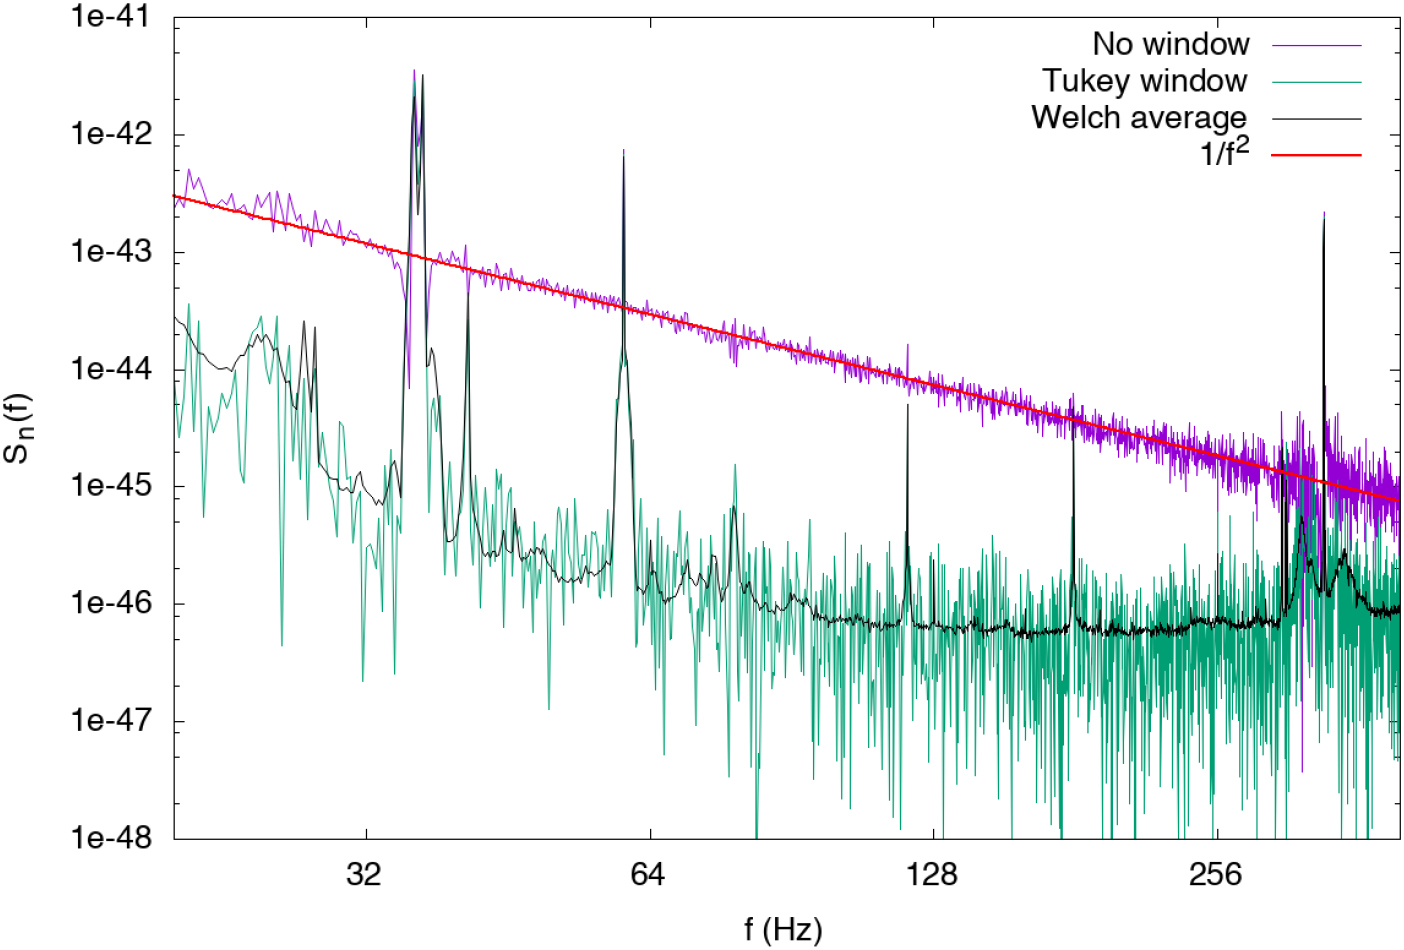
\includegraphics{img/4.jpg}
    \caption{
        图 3 所示数据的功率谱密度. 非窗数据的光谱被光谱泄漏淹没, 并遵循$ 1/f^2$缩放. Welch平均值是使用较长的数据计算得出的. 
    }
\end{figure}

当噪声频谱随时间发生显著变化时, 必须使用其他频谱估计方法[20,66].  LVC参数估计研究中使用的一种方法是将参数化光谱模型拟合到具有平滑样条分量和Lorentzian线集合的数据中[64]. 在第 5 节中, 我们还详细讨论了数据的稳态性和非稳态性问题, 以及这对数据分析的影响. 

除了会导致频谱泄漏外, 数据窗化不当还会导致Fourier变换中的虚假相位相关性. 图 5 显示了图 4 所示的相同数据段的Fourier相位散点图与频率的函数关系, 无论是否应用窗函数. 未开窗的数据显示出很强的相位相关性, 而开窗数据则没有. 
\begin{figure}[htbp]
    \centering
    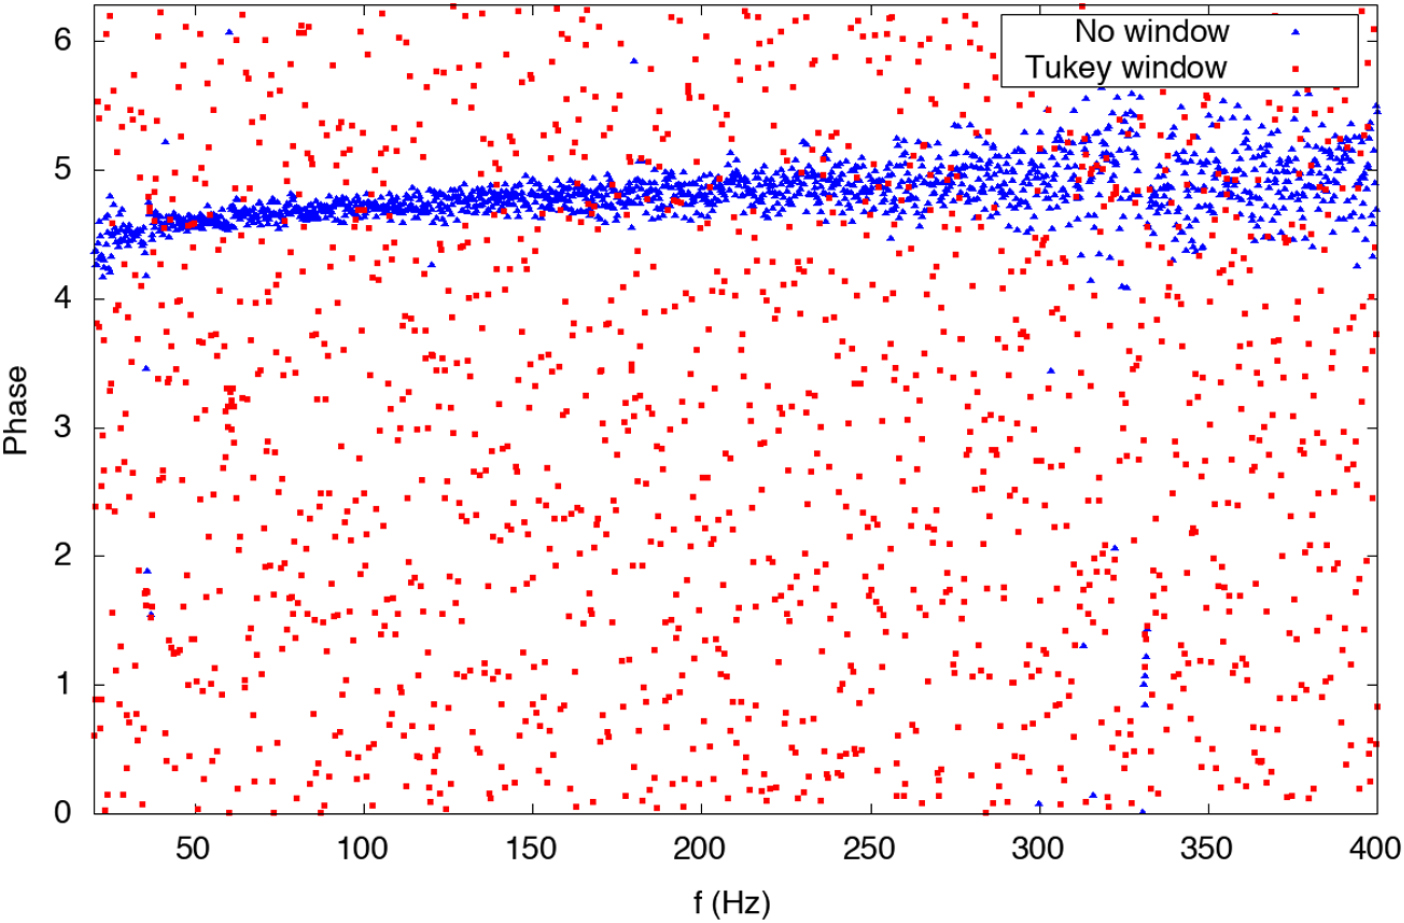
\includegraphics{img/5.jpg}
    \caption{
        LIGO-Hanford数据拉伸的Fourier相位如图3所示. 如果在执行FTT之前未应用任何窗, 如[42]中的分析情况所示, 则光谱泄漏会导致相位相关. 当应用Tukey窗时, 相位看起来是随机分布的, 正如Gaussian噪声所预期的那样. 这些阶段显示围绕$60\t{Hz}$功率线, 与该噪声分量的确定性来源一致. 
    }
\end{figure}

时间序列与稳态噪声和Gaussian噪声的一致性程度可以通过查看其Fourier变换频率样本的分布来诊断. 如果噪声是稳态的和Gaussian的, 则每个频率分档中白化噪声的实部和虚部将是均值和单位方差为零的独立同分布 (i.i.d.)  的随机变量的集合: $x\sim\mathcal{N}(0,1)$. 偏离稳态会导致不同Fourier统计堆栈中的样本之间存在相关性, 而偏离Gaussian的可以通过将样本分布与单位正态分布进行比较来识别. 响亮的仪器噪声瞬态和响亮的引力波爆发确实有助于非稳态和非Gaussian特征, 但远离这些瞬态扰动, LIGO-Virgo数据可以近似为稳态和Gaussian. 图6显示了LIGO-Livingston天文台一段安静数据的白化Fourier振幅. 
\begin{figure}[htbp]
    \centering
    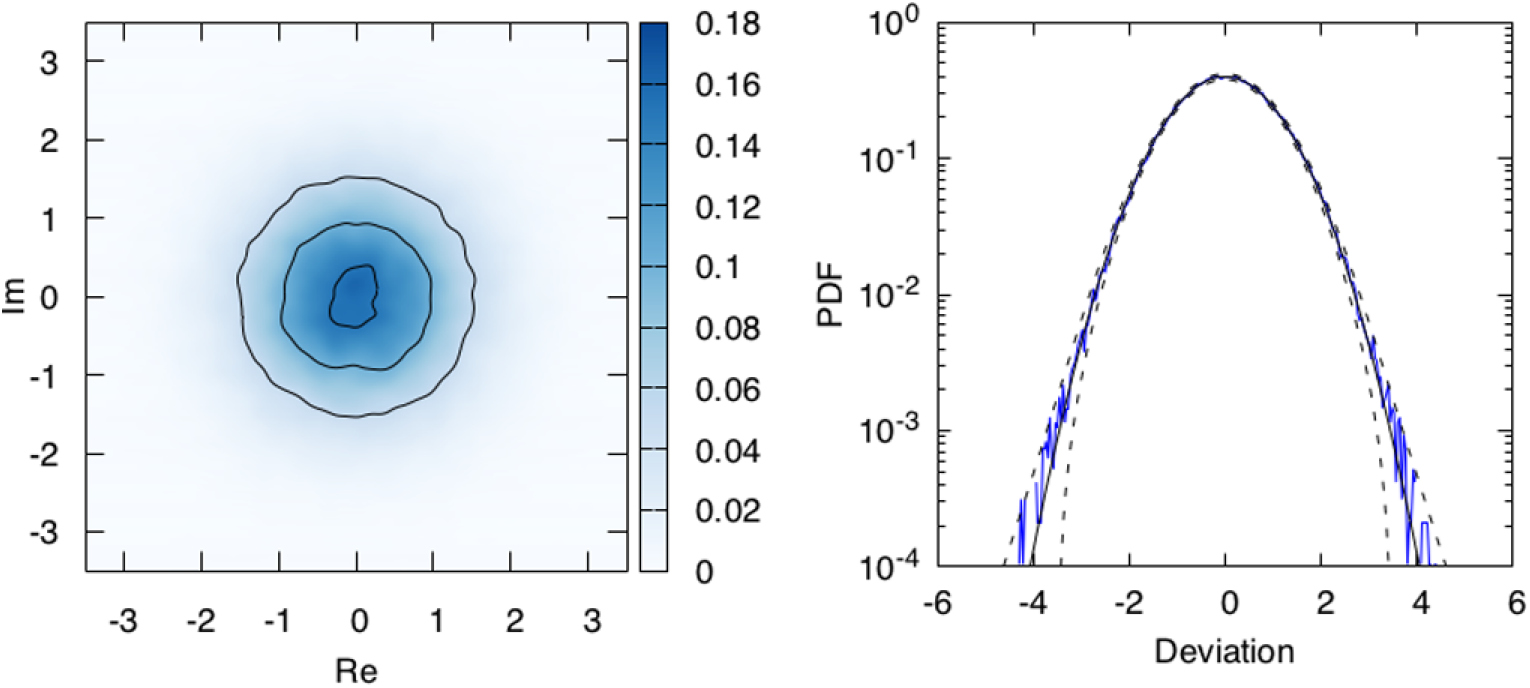
\includegraphics{img/6.jpg}
    \caption{
        左侧的子图显示了使用$256\t{s}$的LIGO-Livingston数据的白化实数和虚数Fourier振幅偏差的二维密度图, 该数据覆盖从$32\t{Hz}$到$512\t{Hz}$的波段且以GPS时间1186741733为中心. 右侧子图显示了Fourier振幅的一维直方图. 实线是给$\mathcal{N}(0,1)$分布的一个参考, 而虚线表示具有有限数量的样本所导致的预期 3-$\sigma$ 方差. 
    }
\end{figure}

\section{时频分析和稳态性}

LIGO-Virgo数据表现出两种主要类型的非稳态行为. 第一种是功率谱中在几分钟或几小时内发生的缓慢而连续的绝热漂移, 第二种是短时噪声瞬变, 我们称之为毛刺 (glitch), 毛刺通常在时间和频率上是局部的. 在光谱线附近还观测到额外的非稳态性, 例如由于电磁耦合到 $50/60 \t{Hz}$ 交流电源而产生的非稳态性. 功率谱中的绝热漂移可以用局部稳态过程来定义[67,68].  局部稳态过程具有协方差函数, 它是稳态过程的协方差函数和时间变量函数的乘积. 

数据的稳态性作为候选事件验证的一部分进行评估[3,48]. 在这里, 我们描述了一些可以应用于数据的简化非稳态性检验. 原则上, 非稳态性可以通过寻找Fourier振幅的相关性来识别, 但使用时频方法更容易识别和分类非稳态行为. 最简单的方法是将数据划分为以时间$ t_i $为中心的小时间块, 并计算每个块的功率谱的平滑估计值$S_n(f, t_i)$.图7显示了Bayesian 功率谱密度估计值[64], 该估计值使用LIGO-Hanford仪器的$8\t{s}$数据段计算得出, 这些数据间隔为$64\t{s}$. 在此期间, 仪器噪声水平变化很大, 在$32 \t{Hz}$和$256 \t{Hz}$之间的频段内, 功率谱密度发生了很大变化 (请注意, 之所以选择此特定时间段, 是因为观测到探测器灵敏度的巨大变化) . 
\begin{figure}[htbp]
    \centering
    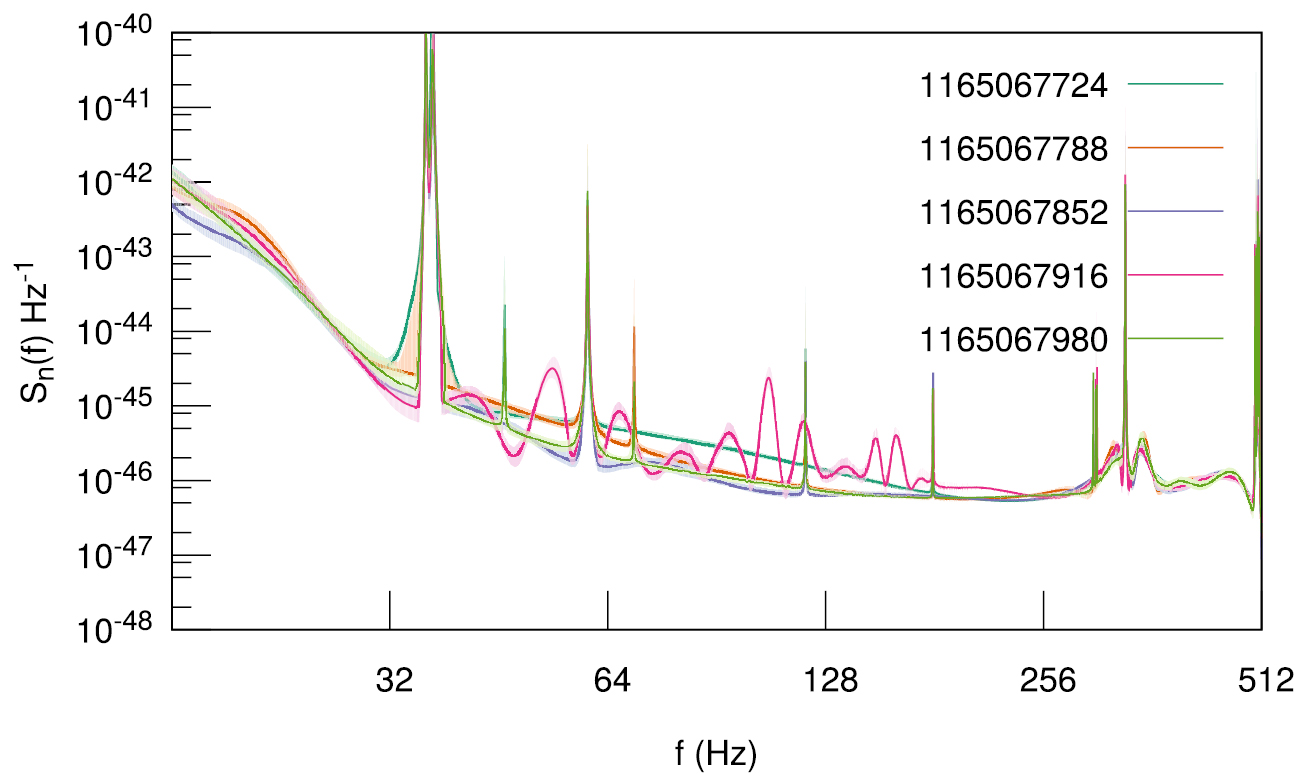
\includegraphics{img/7.jpg}
    \caption{
        LIGO-Hanford探测器的功率谱密度 (实线) 和90\%{}的可信间隔 (阴影带) , 使用从GPS时间1165067724开始的$8\t{s}$数据段 (间隔$64\t{s}$) 计算得出. 在此期间, $32$ 至 $256 \t{Hz}$ 之间存在显着的宽带非稳态性. 
    }
\end{figure}

小波提供了比短时Fourier变换更灵活的分析框架. 连续小波变换通常用于LIGO-Virgo数据研究中, 以产生提供非稳态行为视觉指示的频谱图. 也可以通过使用离散的正交小波变换来对非稳态性进行定量评估. 这些可以使用标尺图来可视化, 显示每个离散时间和频率像素上小波基函数的幅度. 图8显示了用于生成图7的同一段LIGO-Hanford数据的尺度图. 首先使用从以 GPS 时间为 1165067917 为中心的 $256 \t{s}$数据中获取的振幅光谱密度估计值对数据进行白化. 然后使用离散波包\footnote{请注意, 标准离散小波变换按特定顺序应用连续的高通和低通滤波器. 小波波包变换对此进行了推广, 以考虑滤波器应用顺序的所有可能组合. 通过此转换序列的特定路径定义了一些小波波包转换. 人们可以自由选择分解路径. 可以使用各种标准来为特定数据集选择最优或接近最优的分解. 在本文介绍的研究中, 我们使用了一种在频带中给出规则间距的路径, 因为这种选择提供了离散Fourier变换对更灵活的时频情况的简单推广. 有关此方法的更多信息, 请参见[69]. }对白化数据进行转换, 该波包由Meyer小波[70]构建, 这些波包被选择去提供大小$\Delta t=0.5\t{s}$ 和$\Delta f=1\t{Hz}$的平铺的均匀时间和频率覆盖. 然后, 通过将 $16$ 到 $256 \t{Hz}$ 之间的小波振幅的平方相加 (并除以归一化常数) 来计算每次的平均功率. 噪声水平在数据段中心周围近一分钟被提高. 
\begin{figure}[htbp]
    \centering
    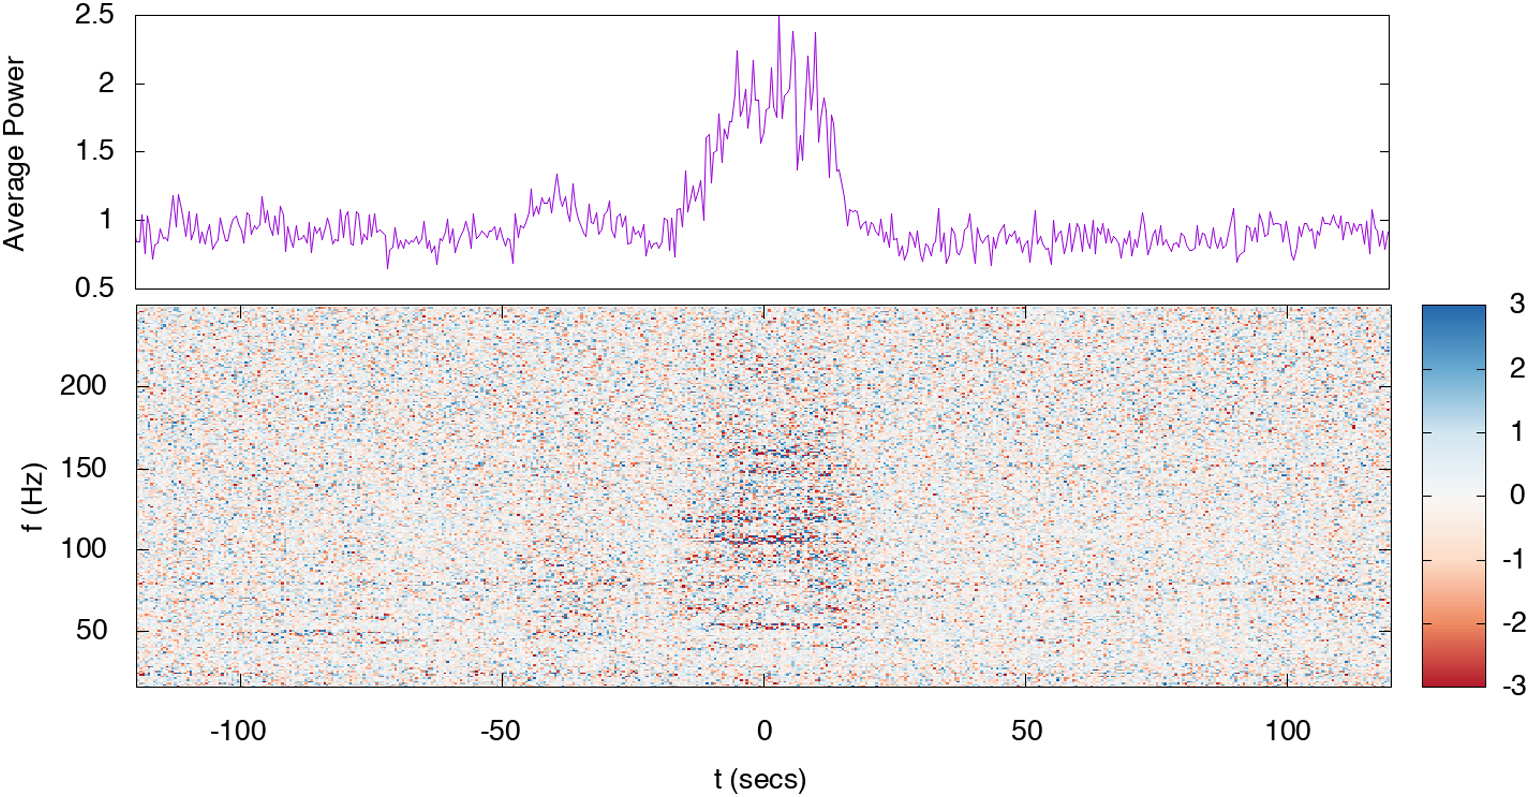
\includegraphics{img/8.jpg}
    \caption{
        用于生成图7的同一段高度非稳态的LIGO-Hanford数据的白化数据的波动. 首先使用从GPS时间1165067917为中心的$256 \t{s}$数据估计的振幅谱密度对数据进行白化, 然后使用离散小波波包变换来生成下图所示的标尺图. 上子图显示了从标度图计算出的时间与时间的函数关系. 
    }
\end{figure}

当此分析应用于稳态Gaussian噪声时, 每个时间间隔内的功率都遵循具有 $N_f$ 自由度的$\chi$方分布, 其中  $N_f$是相加的频率像素数. 可以使用Anderson-Darling检验[71]将平均功率的分布与该参考分布进行比较, 以产生非稳态性的定量度量. 请注意, 虽然无论考虑什么时间跨度, 稳态噪声都是稳态的, 但非稳态噪声将根据平均尺度 (此处为小波像素在时间上的宽度) 和数据的时间跨度产生不同的偏离度量. 出于可视化目的, 可以方便地转换平均功率$p(t)$到一个新变量$s(t)$通过Wilson-Hilferty变换[72], 使得$s(t)$遵循一个${{\mathcal N}} (0,1) $的Gaussian分布当噪声是稳态和Gaussian时. 

将 Anderson-Darling 检验应用于总功率可生成 $p$ 值, 用于数据是稳态的假设. 当应用于图 9 所示的静默数据段时, 检验产生的 $p$ 值为$ p = 0.74$, 表明在此小波尺度下, 数据在此时间段内稳态的假设不能被拒绝. 对图 10 中显示的数据应用相同的检验, 得到的 $p$ 值为$p=2.3\times 10^{-6}$, 我们可以高置信度地拒绝数据是稳态的假设. 任何试图观测或估计在这段数据中可能发生的引力波信号参数的分析都必须采取措施来减轻, 抑制或以其他方式解释与稳态噪声的偏离. 
\begin{figure}[htbp]
    \centering
    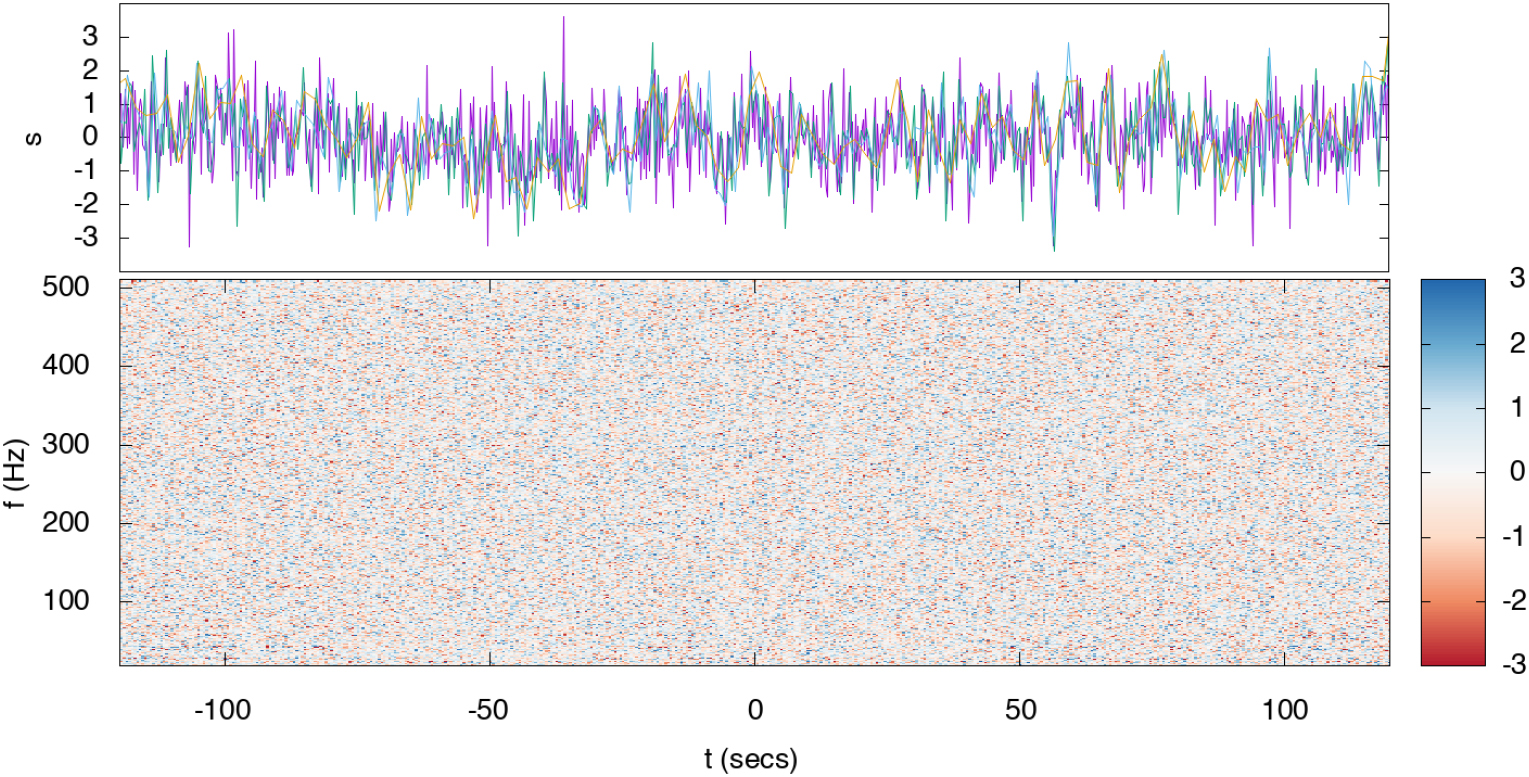
\includegraphics{img/9.jpg}
    \caption{
        来自LIGO-Livingston实验室的一段安静的白色应变数据以GPS时间为1186741733为中心. 上部子图显示转换后的平均功率统计信息$s(t)$适用于各种小波分辨率 (以不同颜色绘制) , 像素宽度范围为 $0.25 \t{s}$至 $2 \t{s}$. 功率波动$s(t)$当噪声是稳态的和Gaussian的时, 应遵循零均值, 单位方差Gaussian分布. 下图显示了分辨率为 $0.5 \t{s}$的小波尺度图. 
    }
\end{figure}
\begin{figure}[htbp]
    \centering
    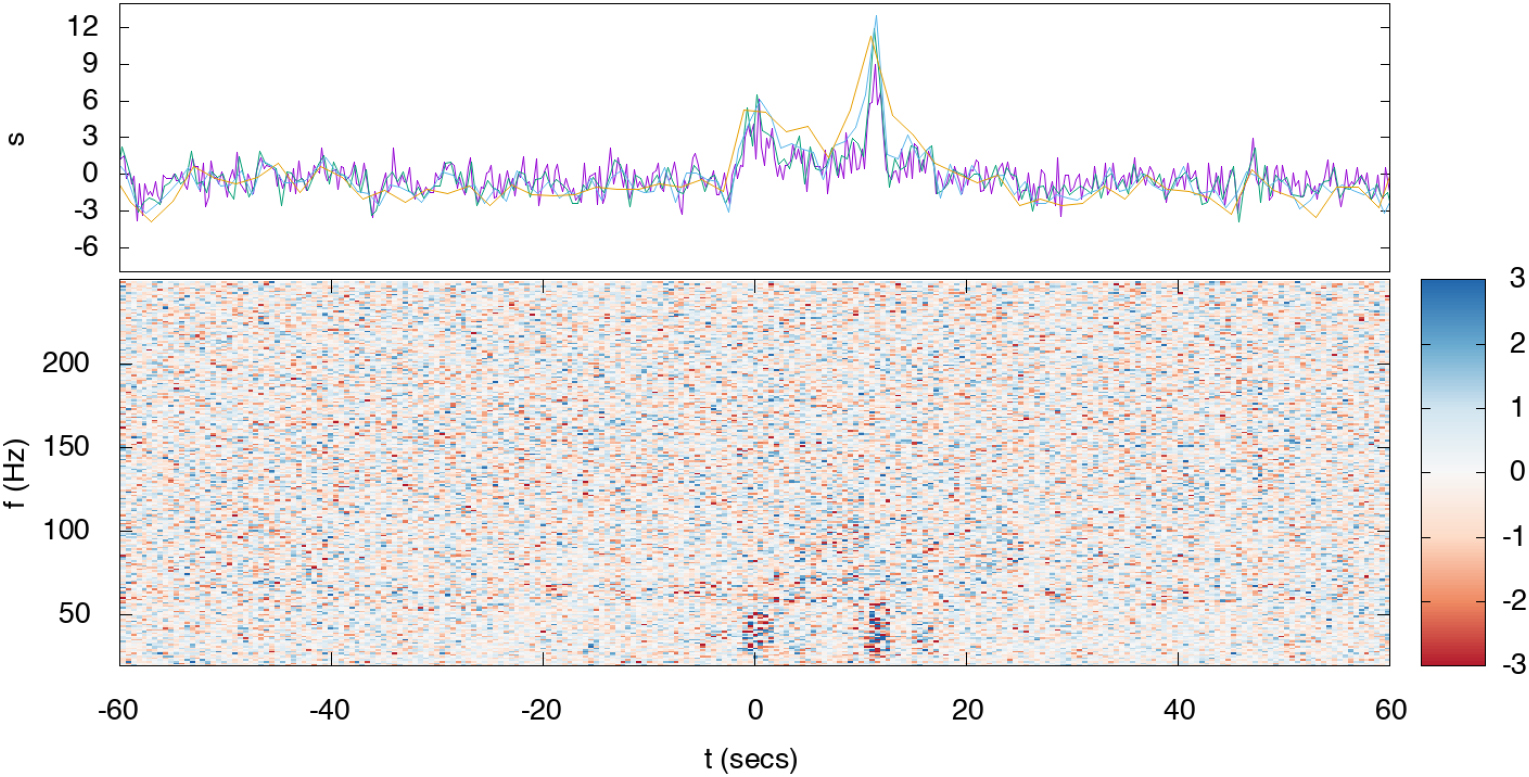
\includegraphics{img/10.jpg}
    \caption{
        LIGO-Livingston实验室的一段白化应变数据以GPS时间为1166358283为中心. 上部子图显示转换后的平均功率统计信息$s(t)$适用于像素宽度范围为 $0.25 \t{s}$至 $2 \t{s}$的各种小波分辨率. 功率波动$s(t)$当噪声是稳态的和Gaussian的时, 应遵循零均值, 单位方差Gaussian分布. 下图显示了分辨率为 $0.5 \t{s}$的小波尺度图. 一系列毛刺会导致显著的非稳态性. 
    }
\end{figure}

\section{探测器标定和数据质量}

在本节中, 我们将提供与数据标定相关的中心概念, 以及我们执行的数据质量检查的概述. 这些程序确保用于分析的应变数据 (即 LVC 在公布结果中使用的分析) 和在 GWOSC 上公开的应变数据使用已知的误差线进行正确标定, 并且可以避免数据质量差的时间段, 如下所述. 

\subsection{探测器标定}

Advanced LIGO [9,  55,  73,  74] 和 Advanced Virgo [10,  47,  75] 探测器使用反馈回路来保持光腔的共振. 因此, 应变标定必须包括所有读出电子设备的模型和测量值, 以及通过悬挂系统中的多个点作用在镜子上的驱动硬件的电子设备和传递函数的模型和测量值[76]. 如图11所示, Advanced LIGO的差分臂控制环路有三个主要组成部分:驱动函数$A (f) $, 感应函数$C (f) $, 以及应用的数字滤波器, $D (f) $.这三者都是作为频率函数进行测量和建模的. 
\begin{figure}[htbp]
    \centering
    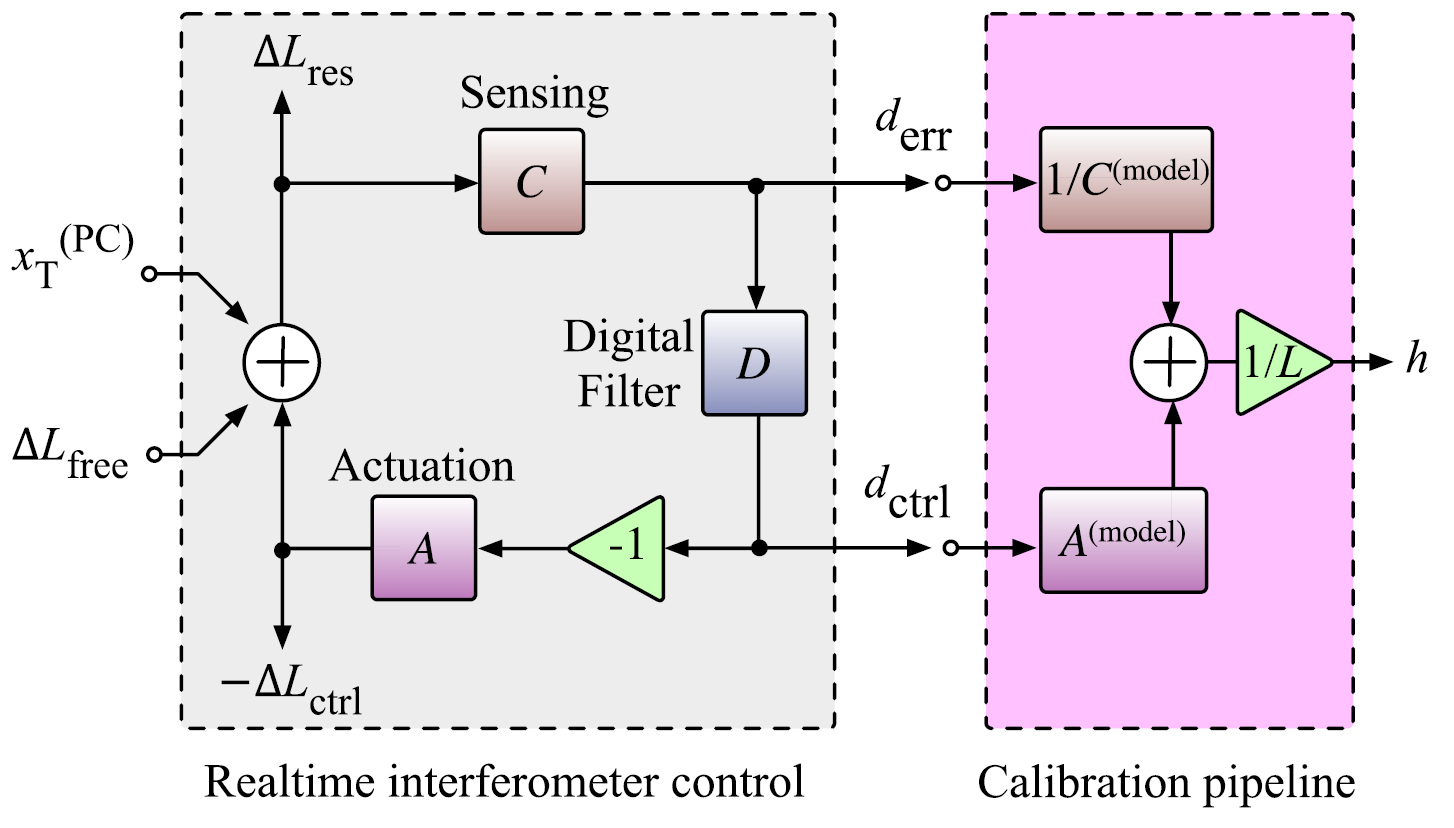
\includegraphics{img/11.jpg}
    \caption{
        LIGO探测器的差分臂长控制回路和标定图, 摘自GW150914一篇关于标定的配套论文[55]. 左侧 (灰色) 框显示实时探测器控制, 右侧 (紫色) 框显示标定程序. $\Delta L_{\t{free}}$是差分臂长度的未抑制变化, 因此是所需的量. 光电二极管 (感应 $C$ 的一部分) 测量残余差分臂长度$\Delta L_{\t{res}}$, 这被反馈回路抑制. ``错误信号''$d_{\t{err}}$, 等于$\Delta L_{\t{res}}$乘以感应函数$C$, 通过数字滤波器$D$, 再通过驱动函数$A$施加到差分臂长度驱动器上. 为了重建$\Delta L_{\t{free}}$在应变单位中, 我们建模 $A$ 和 $C$, 用紫色框表示. $x_{T}^{ (PC) }$表示在回路中, 我们通过辐射压力 (光子标定器) 向测试质量镜施加力, 以便测量 $A$ 和 $C$, 作为频率的函数. 标定管道的输出是应变信号, $h(t)$, 这是对$\Delta L_{\t{free}/L}$的准确可靠表示.
    }
\end{figure}

众所周知, 数字滤波器具有很高的精度, 因此标定误差和不确定度来自模型与驱动和传感函数 ($A$和$C$) 的测量值 (包括测量误差) 之间的差异. 为了独立测量驱动和传感函数, 来自辅助激光器的一对光束从每个测试质量镜反射出来, 它们的强度以已知的频率和振幅进行调制, 以在辐射压力下驱动. 这些辅助激光器组件被称为光子标定器[77]. 一旦知道 $A$ 和 $C$, 真正的差分臂长度就被提取出来, 并通过除以臂 $L$ 的公共长度 (LIGO 为 $4 \t{km}$, Virgo 为 $3 \t{km}$) 转换为应变, 根据以下等式:
\begin{equation}
    h(t)=\frac{1}{L}\left[\mathcal{C}^{-1}\ast d_{\t{err}}(t)+\mathcal{A}\ast d_{\t{ctrl}}(t)\right],
\end{equation}
其中$\mathcal{C}$和$\mathcal{A}$是从驱动函数的频域测量$A (f) $和传感函数的频域测量$C (f) $得出的时域滤波器.

请注意, 引力波应变也可能出现在共模臂长度变化中, 以及探测器中所有自由度长度的变化中. 然而, 只有对干涉仪臂长差分变化的感测才被设计为具有足够低的仪器噪声, 以便对引力波引起的应变敏感. 控制其他光学长度, 以便在微分自由度中保持对引力波应变的最佳线性响应. 

在每次观测运行中定期进行标定测量. 此外, 为了监测光学增益, 腔极点频率和驱动强度漂移等时间相关参数, 通过使用光子标定器在测试质量镜上施加正弦力, 在特定频率下连续注入几条标定线;这些线将出现在原始应变数据中. 探测器之间的标定线频率不同. 

对于第二次观测运行 O2 及以后, 将从标定线中删除标定线$h(t)$应变数据通道 (标定精度以内) [47,78]; 未从O1数据中删除标定线[74]. 即使对于O1, 标定线的存在也不会影响对紧凑双星聚结引力波信号的搜索, 因为在计算每个探测器的数据的探测统计量时, 线频率处的数据振幅通过数据的白化[79,80]被抑制 (见第8节) .  同样, 对于参数估计, 似然中噪声频谱密度的存在 (参见第9节) 可以最小化包括标定线在内的频谱线的影响. 由于频谱线较窄, 因此这种频域加权对信号搜索和参数估计的影响可以忽略不计, 并且不会导致任何杂散效应, 例如生成错误的候选事件或参数偏差. 

对于 O2 中的Advanced Virgo 标定, 有必要考虑干涉仪光学响应的传递函数. 这需要对反射镜的纵向致动器进行标定, 仍然基于激光波长作为长度参考, 使用[81]中描述的所谓自由摆动Michelson配置. 此外, 由读出电子设备确定的干涉仪的输出功率也需要标定. 在每次观测运行中每周进行一次标定测量, 并显示出稳定的驱动强度. 为了监测瞬态光学增益和腔极点频率, 通过使用电磁致动器在测试质量镜上施加正弦力, 在特定频率下连续注入几条标定线, 就像在LIGO探测器中一样. 通过构造, 标定线从标定线中移除$h(t)$应变数据通道 (在标定精度范围内) . 对于 O2 中的Advanced Virgo, 引力波应变重建消除了控制信号对测试质量镜像运动的贡献. 使用光子标定器, 即辅助激光器, 用于反射镜子上的光子并诱导动量传递, 以验证标定并确认应变通道的标志$h(t)$.参见 [47] 了解 O2 Advanced Virgo 标定系统的更多细节. 

LIGO和Virgo探测器的标定应变数据是在线创建的, 用于低延迟搜索. 在完成观测运行后, 为每个探测器生成最终的瞬态标定. GWTC-1 [3] 中给出的结果使用了 [47,  82,  83] 中描述的全频率相关标定不确定度. 需要注意的是, 探测器应变通道$h(t)$Advanced LIGO仅在$10 \t{Hz}$和$5 \t{kHz}$之间标定, Advanced Virgo仅在$10 \t{Hz}$和$8 \t{kHz}$之间标定[47]; 该通道不能准确可靠地表示较低或较高频率下的应变. 

\section{数据质量和地球噪声}

如第3节和第5节所述, 标定的LIGO和Virgo数据在特定时间和频率下可以既是非稳态的也是非Gaussian的. 毛刺可能会在单个探测器中模仿真正的瞬态天体物理信号[48], 而像图2所示的光谱线可能会盲目搜索这些特定频率下的长时间信号[49]. 在本节中, 我们概述了如何识别和表征这些噪声特征, 以便我们可以排除不良数据或评估剩余伪影对搜索引力波信号的影响. 

图 12 显示了一个毛刺示例. 历史上, 功率与可观测信号相当的毛刺大约每分钟发生一次, 较大的毛刺发生频率较低. 即使在其标称状态下, 探测器的数据也包含由仪器行为或仪器与其环境之间的复杂交互引起的毛刺. 其中许多毛刺 (但不是全部) 可能与来自各种传感器的辅助通道中的瞬态信号有关, 这些传感器充当耦合到干涉仪的环境干扰的``见证者''. 这些关联使我们能够识别和编目某些类别的故障. 参见[48], 详细介绍了Advanced LIGO中瞬态噪声的表征, 特别是与观测引力波信号GW150914有关的. O2中Advanced Virgo的各种噪声源的描述可以在[84-87]中找到. 
\begin{figure}[htbp]
    \centering
    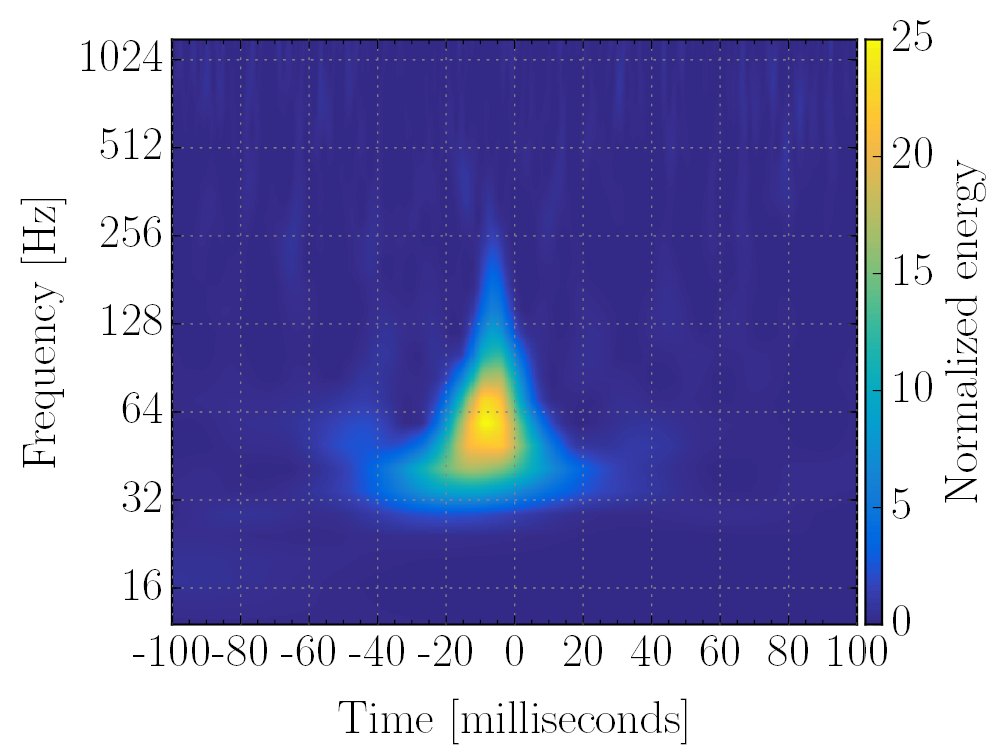
\includegraphics{img/12.jpg}
    \caption{
        高级检波器中瞬态噪声示例的频谱图; LIGO-Livingston的一个尖短毛刺. 这是图10的[50]中所示的尖短毛刺的放大图像. 
    }
\end{figure}

在搜索瞬态引力波信号时, 会标记出已识别的毛刺和数据质量差的时期[50,88,89]. 根据问题的严重性, 在不同级别或类别的数据周期被否决; GWOSC的公开数据发布提供了这些信息[24]. 会破坏噪声功率谱密度估计的强非稳态数据部分将从搜索中完全删除. 当已知物理耦合到探测器的引力波应变通道的噪声源处于活动状态, 从而可能导致毛刺时, 会被识别出来, 并且在这些时间或前后的候选噪声源可能会从搜索结果中删除 (否决) . 有关减轻噪声源的策略的更详细说明, 请参阅[48]的第4节. 对于长时间信号的搜索, 分析中省略了已知以仪器噪声为主的频段[49]. 否决可能毛刺时间的策略有望提高在否决权应用后幸存下来的探测候选物的置信度[50,90,91], 从而可能增加可以自信地观测到的天体物理信号的数量. 第8节将详细讨论观测方法. 

尽管绝大多数瞬态噪声源是本地来源的, 因此在探测器之间不相关, 但存在一些噪声源, 它们在探测器之间可能相关, 例如来自雷电的电磁脉冲感应耦合到探测器中[92]. LIGO和Virgo实验设计的一个关键特征是一系列物理环境监测器, 旨在观测环境干扰, 并且比探测器的引力波应变通道对这些干扰具有更高的灵敏度. LIGO环境传感器阵列包括地震仪, 传声器, 加速度计, 无线电接收器和磁力计, 用于监测环境噪声[93]\footnote{另请参阅\href{http://pem.ligo.org}{http://pem.ligo.org}}.  Virgo也有类似的传感器阵列[10]\footnote{另请参阅\href{https://tds.virgo-gw.eu/?content=3&r=15647}{https://tds.virgo-gw.eu/?content=3\&{}r=15647}}. 环境传感器的灵敏度通过在每次观测运行开始和结束时执行的一套噪声注入来验证; 进行声学, 磁学, 射频和振动测试, 以量化环境噪声与引力波应变数据$h(t)$的耦合 [48]. 这些进样在探测器周围的多个位置进行, 使得通过多个电位耦合路径到$h(t)$的传感器函数能够得到验证和理解. 

如图[48]的图2所示, 环境噪声与引力波数据通道$h(t)$的外部瞬态电磁耦合大约比当前应变水平低 100 倍, 因此任何电磁源都必须在探测器周围的磁力计之一中记录 100 的 SNR, 然后才能在引力波信号通道中记录. 通过对附近风暴期间雷击的研究, 可以很容易地证实这一点[48]. 探测器输出应变信号$h(t)$之间的相干性描述关于交流电源频率 ($50/60 \t{Hz}$) 的探测器的磁力计是非微不足道的, 并在[94]中进行了描述. 在Virgo, 最近对电磁耦合与引力波数据通道进行了详细的研究[84,85]. 

此外, 在寻找随机引力波背景时, 一个潜在的相关噪声源是Schumann共振, 即地球表面与由闪电激发的电离层之间的低频磁场共振[95,96].  这些共振也通过灵敏的磁力计进行监测, 未来的目标是减去它们对引力波应变数据的影响[97]. Schumann共振对测量的引力波应变的影响低于当前的Advanced LIGO-Advanced Virgo噪声基底[98]. 

\section{噪声模型和似然函数}

引力波应变数据包含给定信号的似然函数是引力波事件观测和参数估计的中心量. 在本节中, 我们将这种似然函数与通常对引力波探测器应变数据的噪声分量进行的模型假设进行了关联. 从一台干涉仪中收集的数据时间序列${\b {d}}$可以写成探测器的引力波响应, $\mathfrak{h}$, 和该检波器中所有噪声源的组合${\b {n}}$的和因此是${\b{ d}}={\b {n}}+\mathfrak{h}$. 由于探测器中的真实引力波信号$\mathfrak{h}$是未知的, 我们求助于使用由$\b{h}$表示的信号模型.我们考虑一个模型$\b{h}$要很好地描述数据中的信号, 如果残差${\b {r}} = {\b {d}} - \b{h}$与我们的仪器噪声模型一致. 更定量地说, 数据${\b {d}}$包含可能的信号$\mathfrak{h}$的似然函数由以下概率给出:${\b{ r}}$是噪声模型的实现. 换句话说, 似然函数就是噪声模型. 对于Gaussian噪声, 似然函数可以写成:
\begin{equation}
    p(\b {d}\mid\b{h})=\frac{1}{\mathrm{det}(2\pi\b{C})^{1/2}}e^{-\frac{1}{2}\chi^2(\b {d},\b{h})},
\end{equation}
其中${\b {C}}$是噪声相关矩阵, 并且
\begin{equation}
    \chi^2(\b {d},\b{h})=\b{r}\cdot\b{C}^{-1}\cdot\b{r}=(d_{Ik}-h_{Ik}){C}^{-1}_{(Ik)(Jm)}(d_{Jm}-h_{Jm}),
\end{equation}
重复的指数包括探测器网络$I$,  $J$以及数据样本$ k$ 和 $m$的总和. 如果探测器之间的噪声不相关那么$C_{ (ik)  (Jm) } = \delta_{IJ} S^I_{km}$, 其中 $S$ 是噪声频谱密度. 此外, 如果噪声是稳态的, 因此相关性仅取决于数据样本之间的时间滞后, 则每个探测器中的噪声相关矩阵将在Fourier域中呈对角:$S^{I}_{km} = \delta_{km} S^{I} (f_k) $. 在这种情况下, 我们有$\chi^2 ({\b {d}} ,  {\b {h}})  =  ({\b {r}} \mid{\b {r}}) $, 其中$ ({\b {a}} \mid{\b {b}}) $是大家熟悉的噪声加权内积:
\begin{equation}
     ({\b {a}} \mid{\b {b}}) =2\int_0^\infty\frac{\ti{a}(f)\ti{b}^\ast+\ti{a}^\ast(f)\ti{b}}{S_n(f)}\,\d f.
\end{equation}
似然函数  (6)  是 Bayesian 推理 [99] 的核心, 并且通过对信号和噪声模型的先验 [100] 的规范, 可以计算模型证据 [101,  102] (给出信号存在的几率) 和模型参数, $\b{\theta}$, 例如二进制系统的质量和自旋[103-105], 的后验分布, . 对于检波器之间不相关的稳态Gaussian噪声, 似然函数的形式为:
\begin{equation}
    p(\b {d}\mid\b{\theta})=\exp\left(-\frac{1}{2}\sum_I\left[({\b {d}_I} - \b{h}_I(\b{\theta})\mid{\b {d}_I} - \b{h}_I(\b{\theta}))+\int\ln(S_n^I(f))\,\d f\right]\right),
\end{equation}
其中总和是遍及网络中的探测器, 以及$ (a\mid b) $是公式 (8) 中定义的噪声加权内积. 

似然函数也可用于定义由数据中存在和不存在一个信号$\b{h}$之间的似然比给出的频率学派观测统计量 [53,  106]. 如果数据是稳态的和Gaussian的, 则此统计量将遵循已知分布, 并且可以分析计算事件的误报率. 在实践中, 噪声表现出与稳态性和Gaussian性的偏差, 用于观测和表征信号的方法必须进行修改. 已经开发出健壮的搜索方法, 将噪声的测量特性考虑在内. 这些将在第 8 节中介绍. 第9节介绍了应用于参数估计和信号表征的噪声建模和一致性检查. 

\section{信号探测}

在本节中, 我们将介绍如何在LIGO-Virgo数据中识别候选信号, 以及如何通过与观测到的探测器噪声特性进行比较来量化每个候选信号的统计显著性. 

\subsection{模型比较和匹配滤波器}

LVC对引力波的搜索比较了给定的数据段仅包含噪声的零假设, ${{\mathcal {H}}}_0$, 和该数据段既包含噪声又包含引力波信号的信号假设\footnote{实际上, 所有LIGO-Virgo的数据都可能包含一定程度的引力波信号, 但只有当零假设相对于信号假设足够不利时, 才能观测到信号. }, ${{\mathcal H}}_1$. 大多数搜索都假设广义相对论正确地描述了引力波信号. 在两个假设下观察数据的似然函数可以用公式 (6) 表示成
\begin{equation}
    p(\b{d} \mid{{\mathcal {H}}}_0)=p_0(\b{d})\quad \t{and}\quad p(\b{d} \mid{{\mathcal {H}}}_1)=p_1(\b{d})
\end{equation}
其中${{\mathcal H}}_0$假设数据中没有信号, 只有噪声, 而${{\mathcal H}}_1$假设除了噪声之外还存在由$\b{\theta}$参数化的信号${\b{h}} ({\b{\theta}}) $. 目前, 我们假设每个检波器数据流都被独立分析, 下面我们将讨论来自多个检波器的数据如何在 LVC 搜索中被并合. 给定观测数据的信号假设的概率, 称为后验概率, 由Bayesian定理给出为
\begin{equation}
    p({{\mathcal {H}}}_1 \mid\b{d})=\frac{p({{\mathcal {H}}}_1 )p_1(\b{d})}{p({{\mathcal {H}}}_0 )p_0(\b{d})+p({{\mathcal {H}}}_1 )p_1(\b{d})}=\frac{p_1(\b{d})}{p_0(\b{d})}\left[\frac{p_1(\b{d})}{p_0(\b{d})}+\frac{p({{\mathcal {H}}}_0 )}{p({{\mathcal {H}}}_1 )}\right]^{-1}
\end{equation}
其中$p ({{\mathcal H}}_0) $和$p ({{\mathcal H}}_1) $是我们对数据中不存在或存在信号的先验信念. 无论这些先验信念如何, 后验概率在(如下)似然比中被认为是单调的
\begin{equation}
    \b{\lambda}(\b{d}\mid\b{\theta})=\frac{p(\b{d} \mid{{\mathcal {H}}}_1)}{p(\b{d} \mid{{\mathcal {H}}}_0)}=\frac{p_1(\b{d})}{p_0(\b{d})}
\end{equation}
因此, 这个量是最优检验统计量[54]. 对于Gaussian噪声, 似然比的对数可以用方程 (8) 的内积写为
\begin{equation}
    \log\b{\lambda}(\b{d}\mid\b{\theta})=(\b{d} \mid\b{h}(\b{\theta}))-\frac{1}{2}(\b{h}(\b{\theta}) \mid\b{h}(\b{\theta}))
\end{equation}
此表达式只有第一项涉及数据; 然后观察到后验概率是$ ({\b{d}} \mid {\b{h}} (\b{\theta}) ) $的单调函数, 这个量称为匹配滤波器, 因此, 这个量也是一个最优检验统计量. 

\subsection{信噪比和模板库}

在对引力波信号进行匹配滤波器搜索时, 信号参数$\b{\theta}$不会事先知道. 最优观测统计量可以通过通过将似然比对这些参数\footnote{获得最优统计量的积分度量由引力波信号在未知参数上的概率密度给出[108]: 例如, 如果参数$\b{\theta}$包括$\iota$, 对于紧凑的双星引力波源双星轨道相对于视线的倾角, 那么在$\iota$上的信号概率密度是在$\cos \iota$ 中均匀的[109]. }进行积分来边缘化[107]似然比$\b{\lambda} (\b{d}\mid\b{\theta}) $来获得. 

由于对数似然比是信号模型的线性函数, 因此其指数 (似然比本身) 通常会在其最大值附近急剧达到峰值, 因此$\b{\lambda} (\b{d}\mid\b{\theta}) $的未知参数$\b{\theta}$上的最大值预计可以很好地近似于边缘化似然比 (最多有一个可能的常数重缩放) . 这种最大化过程等同于最小化观测器中看到的残差, 如下所示. 对数似然比可以写成
\begin{equation}
    \log\b{\lambda}(\b{d}\mid\b{\theta})=-\frac{1}{2}(\b{d}-\b{h}(\b{\theta}) \mid\b{d}-\b{h}(\b{\theta}))-\frac{1}{2}(\b{d} \mid\b{d})).
\end{equation}
现在很明显, 最大化对数似然比的参数$\hat{\b\theta}$是就噪声加权内积而言最小化残差$\b{d}-\b{h}(\b{\theta})$的参数. 

参数${\b{\theta}}$描述在探测器中观察到的应变, 包括在探测器中观察到的信号振幅$A$ (它与到引力波源的距离成反比) , 在探测器中观察到的正弦变化信号中的相位$\phi$, 信号的到达时间$t$ (通常由探测器处达到峰值引力波振幅的时刻定义) , 和其他描述源的物理参数的参数$\b{\mu}$, 例如成员的质量和自旋. 我们写下
\begin{equation}
    \b{h}(\theta)=A\b{p}(t,\b{\mu})\cos\phi +A\b{q}(t,\b{\mu})\sin\phi
\end{equation}
其中$\b{p}(t,\b{\mu})$和$\b{q}(t,\b{\mu})$是同相 (余弦) 和正交相 (正弦) 波形, 经过归一化处理从而$ ({\b{p}}\mid{\b{p}}) = ({\b{q}}\mid{\b{q}}) =1$, 并且是正交的, $ (\b{p}\mid\b{q}) =0$.

振幅和相位的最大化可以按以下代数方式进行:等式  (13)  可以使用等式  (15)  重写为
\begin{equation}
    \log\b{\lambda}(\b{d}\mid\b{\theta})=A\rho(t,\b{\mu})\cos(\phi-\varphi)-\frac{1}{2}A^2
\end{equation}
其中
\begin{equation}
    \varphi\equiv\arctan\frac{(\b{d}\mid\b{q}(t,\b{\mu}))}{(\b{d}\mid\b{p}(t,\b{\mu}))}
\end{equation}
且
\begin{equation}
    \rho(t,\b{\mu})\equiv\sqrt{(\b{d}\mid\b{p}(t,\b{\mu}))^2+(\b{d}\mid\b{q}(t,\b{\mu}))^2}
\end{equation}
是参数$\b{\mu}$的波形模板的 SNR 时间序列. 对数似然比$\log\b{\lambda}$在$\hat{A} = \rho$且$\hat{\phi} = \varphi$时振幅最大为
\begin{equation}
    \max_{A,\phi}\log\b{\lambda}(\b{\theta})\equiv\log\b{\lambda}(t,\hat{A},\hat{\phi},\b{\mu})=\frac{1}{2}\rho^2(t,\b{\mu}).
\end{equation}
此时间序列中的峰值对应于信号最有可能出现的时间. 在信号 (噪声) 假设下, 在存在具有已知功率谱的稳态且Gaussian噪声的情况下, $\rho^2 (t_{{{\t{ peak}}}}, {\b{\mu}}) $遵循具有两个自由度的非中心 (中心) $\chi$方分布. 

SNR时间序列可以方便地用方程 (8) 表示为复数时间序列[66]
\begin{equation}
    z(t,\b{\mu})=4\int_0^\infty\frac{d(f)p^\ast(f,\b{\mu})}{S_n(f)}e^{2\pi ift}\,\d f
\end{equation}
其中$\rho = |z|$且相位$\varphi = \arg (z) $; $\ti{p} (f, {\b{\mu}}) $是同相波形的Fourier变换 (参见公式 15) . 方程  (20)  是 $z(t,\b{\mu})$的 逆Fourier变换
\begin{equation}
    \ti{z}(f,\b{\mu})=4\frac{d(f)p^\ast(f,\b{\mu})}{S_n(f)}\Theta(f)
\end{equation}
其中$\Theta(f)$是 Heaviside 阶跃函数. 

参数 (由$\b{\mu}$表示) , 例如双星成员的质量和自旋, 改变引力波的形态. 为了观测具有很宽的可能质量和自旋范围的信号, 需要生成一个由跨越参数空间的大量信号模板组成的组, 并且组中的每个模板都用作匹配滤波器. 用于最初在数据中查找信号的模板库是在参数空间中具有足够高的密度构建的, 使得真实信号与最佳拟合模板之间的SNR损失小于3\%{}. 有关用于 O1 和 O2 搜索的模板库的更多详细信息, 请参见 [2,  3,  110]. 

应该注意信噪比的一个重要特性:在等式 (20) 中, 可以看出被积数与$\ti{d} (f) /S_{n} (f) $成正比, 因此数据不是简单地被白化 (如果分母是 $S^{1/2} (f) $则本该是此情形) , 但实际上, 频谱中较多的噪声部分 (包括窄线) 在匹配滤波器中被抑制. 等效地, SNR 积分可以看作是将白化数据时间序列与白化模板相关联. 因此, SNR提供了一种自然的方法, 可以对噪声较大的频段降权, 并有效地消除各种线的缺口. 

\subsection {噪声伪影的抑制和候选体排名统计量的构建}

虽然SNR是稳态Gaussian噪声情况下的最优观测统计量, 但瞬态仪器伪影使其成为真实观测器噪声的非最优统计量. 尽管匹配滤波器自然会抑制数据中稳态的噪声特征, 但毛刺可能导致某些模板产生高SNR值[50,111-113]. 我们通过几种不同的方式解决这个问题:
\begin{enumerate}
    \item 如第 6.2 节所述, 我们使用目击者传感器来识别环境或仪器频繁引入毛刺的时间, 我们否决了分析中发现影响搜索性能的这些时间的一部分 [50]. 这些传感器包括那些监测引力波探测器周围物理环境的传感器, 以及那些记录干涉仪内部控制系统内部信号的传感器. 
    \item 我们实施波形一致性测试, 以表征数据${\b{d}}$和模型${\b{n}}+{\b{h}}$的偏差 [20, 21, 66, 114]. 对于来自密近双星并合的信号, 这些测试非常强大, 使我们能够拒绝许多尚未被识别和否决的毛刺, 尽管对于短信号, 这些测试的鉴别能力减弱了[3,20,114,115].  这些信号一致性测试的确切实现在搜索管道之间有所不同, 但都基于以下原则: 如果从数据中减去引力波模型波形以产生残差${\b{d}}-{\b{h}}$, 如果信号假设为真, 则残差应与Gaussian噪声一致. 这些残差在不同的时间或频率间隔内使用匹配滤波器重新滤波, 以确定非噪声样特征是否仍然存在; 这些特征的证据表明, 模型波形${\b{h}}$与数据中的非Gaussian特征匹配度不高, 观测排名统计量被相应降权. 例如, [66,  114] 中描述的一致性检验通过将匹配滤波器划分为 $n$ 个频段来构建$\chi$方检验统计量
    \begin{equation}
        \chi^2=\sum_{i=1}^n\frac{ |({\b{d}}-{\b{h}} \mid \b{p})_i -({\b{d}}-{\b{h}} \mid \b{p})/n|^2 +|({\b{d}}-{\b{h}}\mid \b{q})_i -({\b{d}}-{\b{h}}\mid \b{q})/n|^2}{1/n}
    \end{equation}
    其中$ (\b{a}\mid\b{b}) _i$与等式 (8) 中的内积相同, 但被积量限制在频率区间$f_{i-1}<f<f_{i}$内, 其中 $f_0 = 0 $且$f_n=\infty$. 在这里选择波段, 以便$ (\b{p}\mid\b{p}) _i= (\b{q}\mid\b{q}) _i=1/n$. 如果残差${\b{d}}-{\b{h}}$是Gaussian噪声, $\chi^2$是$\nu=2n-2$自由度的$\chi$方分布的; $\chi^2\gg\nu$的值表示减去模型后数据中剩余的非Gaussian特征. 一个在[20]中被给出重赋权的排名统计量
    \begin{equation}
        \hat{\rho}=\rho\times\begin{cases}
            1 &  \chi^2 \le \nu \\
            \left[\frac{1}{2}+\frac{1}{2}(\chi^2 /\nu)^3\right]^{-1/6} &  \chi^2 > \nu \\
        \end{cases}
    \end{equation}
    对于较大的值降低 SNR 的权重$\chi^2$.[21]中描述了类似的基于时域的信号一致性检验, 并将其纳入似然函数排名统计量中. 
    \item 对于迄今为止公布的所有探测结果, 我们要求在至少两个参数一致的独立探测器中通过匹配滤波来识别引力波信号. 例如, 引力波在每个探测器的到达时间的差异必须不超过探测器之间的最大飞行时间, 例如, LIGO Hanford-LIGO Livingston对的飞行时间为$10 \t{ms}$, 另外增加$5 \t{ms}$, 以解释每个探测器推断的并合时间的不确定性. 在搜索LIGO Hanford-Virgo对 ($27 \t{ms}$光传播时间) 和LIGO Livingston-Virgo对 ($26 \t{ms}$光传播时间) 的同时事件时, 也使用了对重合窗口的$5 \t{ms}$增加[3]. 然而, 现在已经确定了引力波信号的存在和频率, 现在也可以在只有一个探测器工作时进行探测, 并因此这种时间符合性检验不可用[116]. 
\end{enumerate}

LVC采用的基于匹配滤波器的搜索从SNR和波形一致性测试统计量[3]中构造排名统计量. 此外, 在几个探测器中接收到的一个天体物理信号将具有一组共同的参数$\b{\mu}$ (在有限信噪比规定的限制内) , 此外, 在每个探测器中观察到的信号的幅度, 相位和到达时间将由波的传播方向 (即信号在天空中的来源) 和信号的极化状态确定. 由于引力波有两种极化 (在广义相对论中) , 称为$+$极化$\b{h}_+$和$\times$极化$\b{h}_\times$, 探测器 $I$ 上的应变由探测器的天线响应模式$ F_{+,I} $和$F_{\times,I}$给出
\begin{equation}
    \b{h}_I(\b{\theta})=F_{+,I}(\alpha,\delta,\psi,t)\b{h}_+(t-\tau_I,D,\iota,\b{\mu})+F_{\times,I}(\alpha,\delta,\psi,t)\b{h}_\times(t-\tau_I,D,\iota,\b{\mu})
\end{equation}
其中$\alpha$和$\delta$是引力波源的赤纬和赤纬, $D$是到引力波源的距离, $\iota$是双星系统的轨道平面的倾角 (对于圆形轨道和低阶四极矩辐射, 它决定了椭圆度角) , 以及$\tau_I=\tau_I (\alpha, \delta, t) $是信号从地心到探测器的传播时间. 尽管在探测器网络中对引力波进行完全相干的搜索是可能的, 但我们选择在每个探测器中独立执行搜索, 然后要求在不同探测器中看到的触发器具有一致的到达时间和相同的参数${\b{\mu}}$因为这提供了一个强大的毛刺抑制一致性测试, 如上所述. 但是, 也可以进一步满足信号一致性要求. 对于来自圆形双星的低阶四极矩辐射, 在两个探测器中看到的振幅之比为
\begin{equation}
    \frac{A_I}{A_J}=\sqrt{
        \frac{
            F_{+,I}^2\left(\frac{1+\cos^2\iota}{2}\right)^2+F_{\times,I}^2\cos^2\iota
        }{
            F_{+,J}^2\left(\frac{1+\cos^2\iota}{2}\right)^2+F_{\times,J}^2\cos^2\iota
        }
    }
\end{equation}
而到达时间的差异是$t_I - t_J = \tau_I - \tau_J$且相位之差为
\begin{equation}
    \phi_I - \phi_J = \arctan\left(\frac{F_{\times,J}}{F_{+,J}}\frac{2\cos\iota}{1+\cos^2\iota}\right)-\arctan\left(\frac{F_{\times,I}}{F_{+,I}}\frac{2\cos\iota}{1+\cos^2\iota}\right).
\end{equation}
因此, 可以在基于似然函数的排名统计中包含幅度-相位-时间一致性度量[20,50,117]; 这是针对LIGO-Virgo O1和O2数据中引力波信号的最新搜索进行的[3]. 

\subsection{背景估计和观测置信度}

在采取上述减轻噪声瞬态影响的步骤之后, 剩余瞬态在两个观测器中同时发生的可能性 (在考虑信号最大传播时间的时间窗口内, 例如, 两个LIGO探测器为$10\t{ms}$) 并产生较大的联合排名统计值变得极小. 不同的搜索采用不同的方法来衡量这种概率作为排名统计量的函数[50]. 基本方法是检查在每个检波器中观察到的非同步瞬态的统计特性, 并人为地将它们视为同时发生. 

在两个或多个探测器中观察到的任何候选事件的统计显着性通过其误报率进行量化, 误报率是每次由于噪声导致的预期事件率, 该事件将被分配与候选事件相同或更大的排名统计数据. 估计误报率的一种方法是将一个探测器的数据流在时间上移动 (时间间隔大于探测器之间的最大飞行时间) , 然后重复搜索. 然后, 将生成的``时移''巧合视为背景噪声样本. 为了获得联合观测器排名统计信息的概率分布, 需要在不同的时间偏移下进行多次操作. 每个重合触发器都会被分配一个误报率, 该值由具有相等或更大排名统计数据的背景触发器的数量除以搜索时移巧合的总时间得出. 例如, 在[1]中发现, 在LVC采用的两种匹配滤波器搜索中, 产生比GW150914更重要事件的瞬态频率小于每200 000年一次. 

另一种类似的方法是在另一个探测器中 (在引力波的飞行时间内) 没有同时触发器的单探测器触发器累积, 因此可能与引力波信号无关. 然后, 通过从推断的单个观测器分布中随机抽取单个观测器触发器, 并在构建排名统计量时人为地将它们视为同时存在, 从而估计背景 (仅噪声) 假设下排名统计量的分布. 然后可以使用这种背景分布来评估观察到的排名统计值的显着性[21,117]. 这两种确定观测到的引力波候选物显著性的独立方法都对已确定的引力波产生了高度的显著性. 

这些背景估计方法没有考虑探测器之间可能相关的地球噪声源. 因此, 如上文第6.2节所述, 对监测此类噪声源的物理和环境传感器进行了详细检查, 并评估了它们与测量的引力波应变通道的耦合, 以检查候选观测物的有效性. 

LVC还可以在没有特定波形模型的情况下搜索LIGO和Virgo数据[22,118]. 这些搜索首先识别每个探测器数据流中的过功率周期, 然后根据数据流之间的互相关性构建观测统计信息. 再次使用时移分析来评估特定观测统计值的显著性. 在[1]中, 表明在这种通用瞬态搜索中, 产生比GW150914更重要事件的噪声瞬变频率为每8400年一次. 

采用不同方法的多次搜索都发现GW150914是一个非常重要的候选事件, 这一事实增强了我们的信心, 即该事件不是重合瞬态噪声的产物. 此外, 该信号与广义相对论预测的双黑洞系统并合的波形非常匹配. 使用LVC高置信度探测到的前十个双黑洞并合进行的各种测试显示, 与广义相对论模型没有显著的偏差[119]. 

\subsection{搜索灵敏度的测量}

搜索管道的最后一个组成部分是确定搜索对天体物理信号群体的敏感性. 这样做有两个目的:首先, 它提供了一个指标, 通过该指标可以调整搜索以优化其对特定类别信号的观测效率; 其次, 它提供了一种方法, 用于将管道观测到的信号速率解释为群体生成信号的速率. 

搜索管道的灵敏度通常通过 Monte Carlo程序 (参见[120]) 进行测量, 其中将从假设的源群体 (例如, 双星成员质量和自旋的一些分布, 方向角, 到达时间和距离) 中提取的模拟信号添加到真实探测器噪声中, 然后重新运行搜索以确定搜索管道从该群体中观测到的信号的比例. 如果搜索管道产生高于某个选定的排名统计信息阈值的触发器, 则认为观测到了模拟信号. 结果表示为时间平均和总体平均的时空灵敏度$\langle VT\rangle$对于固定的排序统计阈值, 该阈值对应于固定的误报率阈值 (例如, 可以选择阈值为每个世纪的观察值一次误报) . 或者, 也可以采用与阈值无关的天体物理速率估计方法[121-123]. 

\section{ 推断波形和物理参数}

一旦确定了候选引力波信号, 并确定了其重要性, 下一个目标是利用这些数据来推断产生引力波的系统的物理参数[102-105,  124-127]. 引力波的探测以及物理参数的推断依赖于对所寻找信号的一般形状以及噪声分布的了解. 此外, 引力波信号很弱, 因此这些参数的不确定性可能很大, 并且关于这些信号的典型振幅和相位演化的先验假设确实对重建的波形有重大影响. 由于这些原因, 系统的物理参数 (例如质量, 并合对象的自旋) 的推断是在Bayesian 参数估计的框架内完成的. 需要定义的核心元素是引力波信号的模型$M$, 该模型允许根据系统的物理参数值和所谓的背景或先验信息$I$预测信号的形式. 

给定一个模型 $M$, 它依赖于一组参数$\b{\theta}$, 背景信息$I$和一组观测值 (数据) ${\b d}$, 推理是通过应用Bayesian 定理完成的:
\begin{equation}
    p(\b{\theta}|\b{d},M,I)=p(\b{\theta}|M,I)\frac{p(\b{d}|\b{\theta},M,I)}{ p(\b{d}|M,I) } .
\end{equation}
左侧称为后验概率密度函数, 或简称为$\b{\theta}$的后验, 而右侧的三个项是先验概率密度函数 $p (\b{\theta} |M,  I) $, 由等式 (9) 给出的似然函数 $p ({\b d}|\b{\theta}, M I) $, 和证据
\begin{equation}
    p(\b{d}|M,I) =\int\d\theta\, p(\b{\theta}|M,I)p(\b{d}|\b{\theta},M,I).
\end{equation}
在Bayesian 参数估计框架中, 推理被简化为对 的后验计算$\b{\theta}$给定模型 $M$ 和分析假设 $I$, 它唯一地确定了先验分布和似然函数. 

\section{波形模型}

现在让我们关注信号模型 $M$ 的选择. 信号模型 $M$ 确定$h (t;\b{\theta}) $这是计算似然函数的关键. 为了确定性, 我们将专注于参数化形式$h (t;\b{\theta}) $, 通过求解Einstein方程获得. 有关非参数化形式信号模型的讨论, 请参见[128]. 众所周知, Einstein方程组的精确解析解很难获得; 因此, 数据分析就绪的模型要么基于扰动解, 例如Taylor波形族[129]或有效单体波形[130-134], 要么基于混合/现象学方法, 例如Phenom波形族[135-138]. 我们在这里不会进一步讨论波形模型的细节, 但我们将仅限于GW150914的原始分析中采用的两种主要类型的波形. 对于GW150914, [127]中使用的两个模型是SEOBNRv2和IMRPhenomPv2 [127,139].  两种波形模型都是全旋近-并合-铃宕模型, 它们成功地再现了数值波形, 特别是在质量大致相等和自旋幅度适中的区域. 两种模型的主要区别在于自旋动力学的处理. SEOBNRv2 模拟了自旋矢量分量沿轨道角动量方向的动力学, 而 IMRPhenomPv2 还包括对自旋面内分量动力学的有效处理, 因此包括近似的预置动力学\footnote{在发现GW150914时, 还有另一个预设波形模型SEOBNRv3可用, 其中还包括面内自旋分量[140,141].  然而, 最初的分析并未包括该模型的结果, 这些结果在[142]中进行了报道. }. 由于GW150914几乎是一个对峙系统 (轨道角动量矢量指向远离地球) , LIGO仪器对面内自旋分量不敏感, 因此两个波形模型基本上是等同的. 在[143]中, LVC实证表明, GW150914的推断属性对波形模型变化的依赖性相对较弱. [134]中使用的独立有效单体实现和[144]中提出的分析证实了这一发现, 其中将数值相对论解与GW150914数据进行了直接比较. 

\subsection{先验分布}

应用Bayesian 定理 (方程  (27) )所需的最终函数是感兴趣参数的先验概率分布. 这些都是完全表征并合事件期间发射的引力波信号所必需的参数. 对于准圆形轨道, 它们是:
\begin{itemize}
    \item 成员质量 $m_1 $和 $m_2$;
    \item 自旋向量$\vec {S}_1$和$\vec {S}_2$;
    \item 偏振角$\psi$和总角动量$\vec {J}$和引力波的传播方向$\hat{n}$之间的角度$\theta_{jn}$;
    \item 波源光度距离 $D_L$;
    \item 波源赤经$\alpha$和赤纬$\delta$;
    \item 参考相位$\varphi_0$以及参考时间, 通常是引力波应变峰值时间, $t_0$. 
\end{itemize}

必须为所有参数指定先验分布的函数形式. 在某些情况下, 先验分布是通过参数空间的不变性 (对称性) 属性确定的[145];例如, 波源位置的先验$D_L, \alpha, \delta$根据Friedmann-Lema\^{i}tre-Robertson-Walker宇宙学模型, 在宇宙学共动体积中, 波源的数量密度是均匀的, 因此选择. 因此, 概率$p (D_L,  \alpha,  \delta|M I)  \propto dV $并且对于 红移$z \ll 1$退化到$p (D_L,  \alpha,  \delta|M I)  \propto D_L^2 | \cos (\delta) |$. 在不变性参数不适用的情况下, 我们选择简单的先验分布形式, 以便生成的后验易于解释. 相似的参数确定自旋向量的先验$\vec {S}_1,  \vec {S}_2$和方向角度$\psi, \theta_{jn}$在 $0$ 到 $2\pi$之间的方位角范围内保持均匀以及极角的余弦均匀, 范围在 $-1$ 和 $1$ 之间. 关于自旋矢量的大小, 几种可能的先验是可能的, 例如$p (|\vec {S}_i|\mid M, I)  \propto |\vec {S}_i|^2$或$p (|\vec {S}_i|\mid M, I)  \propto 1$. 对GWTC-1目录中事件的主要分析采用了在自旋向量范数上的均匀分布. 对于分量质量 $m_1$ 和 $m_2$, 所选的先验分布是均匀的, 因此$p (m_1,  m_2 |M I)  \propto 1$, 但从下面限制, 以便$m_1, m_2 > 1M_{\odot}$.

\subsection{标定不确定度}

除了探测器噪声引起的不确定性外, 我们的源参数估计的准确性和精度还受到探测器幅度和相位响应不确定性的影响. 出于这个原因, 对数据上的这种不确定性来源进行建模并包含在分析中. 所采用的标定不确定度模型基于对指定频段内幅度和相位误差幅度的经验估计[47,74,82]. 具体而言, 该模型假设要分布的误差值为Gaussian分布, 均值为零, 方差由经验确定的误差大小给出. 然后, 在数据频率空间上使用三阶样条插值来构建标定不确定度曲线. 通常, 这总共引入了$O (10) $每个检波器的附加参数 (一半用于相位不确定度, 另一半用于幅度) , 这些参数与系统的物理参数一起采样. LVC标定模型的技术细节可以在[146]中找到. 

\subsection{数值方法}

因此, 对于准圆形轨道和通用自旋向量, 要推断的参数总数为 15, 对于自旋被迫与轨道角动量对齐的模型, 要推断的参数总数为 11. 在物理参数集中, 我们必须将每个探测器所需的 10 个参数相加, 以指定标定不确定度模型. 因此, 对于典型的三探测器分析, 我们总共对具有通用自旋取向的准循环系统的所有 45 个参数进行采样. 如此高维的参数空间无法用基于网格的方法有效地探索. 因此, 多年来, LVC的成员开发了\texttt{LALInference}随机采样器库[105], 该库实现了两种算法, 并行退火 Markov链Monte Carlo[147]和嵌套抽样( nested sampling)[102]. 并行退火 Markov链Monte Carlo被设计为从多维后验分布 (27) 生成样本, 而嵌套抽样被设计为计算证据方程 (28) 并从后验分布生成样本作为副产品. 更多细节在[105]中给出, 并在其中引用. LVC经常使用其他参数估计管道, 如rapidPE [148]和BILBY [149], 但在其余的讨论中, 我们将重点关注\texttt{LALInference}. 但是, 同样的考虑因素也适用于其他Bayesian 分析方法. 

\subsection{后验分布}

\texttt{LALInference}分析的最终产品是表征引力波波形的所有参数的后验样本. 特别令人感兴趣的是固有参数, 质量和自旋矢量, 的后验, 它们有助于确定并合天体的性质. 对于GW150914, 使用IMRPhenomPv2波形模型测量的探测器帧质量 (即由于宇宙膨胀而导致的红移) 为:$38.5_{-3.6}^{+5.6} M_\odot$和$32.2_{-4.8}^{+3.6} M_\odot$;参见[127]中的表I. 引用的数字是总结完整后验分布的一种极其简洁的方式. \texttt{LALInference}分析的输出是来自完整后验分布的样本. 特别是, 诸如$38.5_{-3.6}^{+5.6} M_\odot$来自对全后验的 15 个物理源参数中的 14 个以及标定参数的边缘化, 以获得一维后验, 然后从中计算出 90\%{} 的可信区域. 当然, 在一维表示中, 不同参数之间的相关性是不可见的. 为了获得更清晰的图片, 多维后验分布有助于显示从分析中提取的信息. 图 13 以分量质量 $m_1$ 和$ m_2$ 的联合二维后验分布为例. 特别是, 左下角的子图显示了组件质量之间不可忽略的相关性. 
\begin{figure}[htbp]
    \centering
    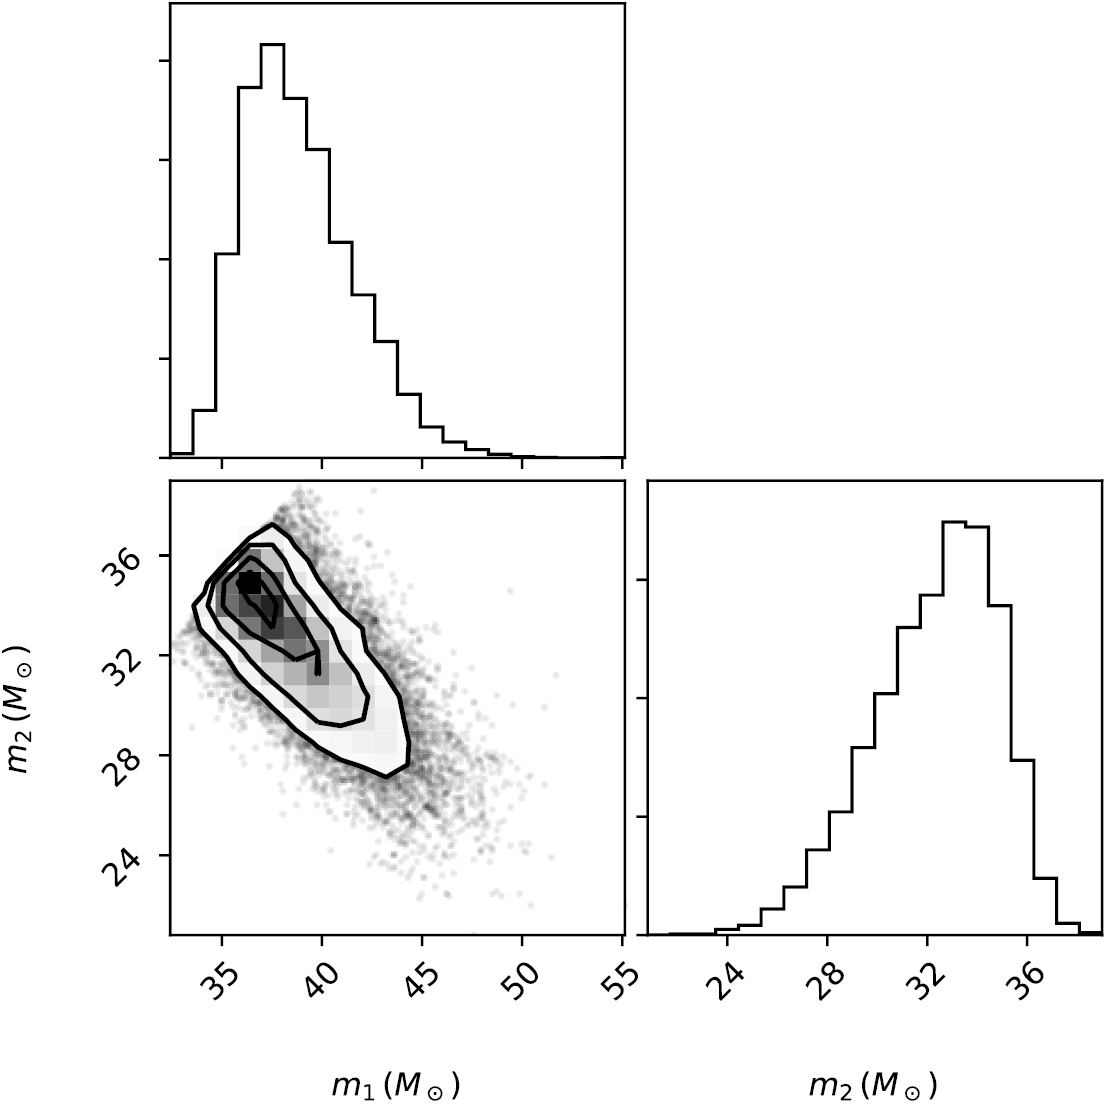
\includegraphics{img/13.jpg}
    \caption{
        使用 IMRPhenomPv2 波形模型获得的GW150914事件的探测器帧质量的一维和二维后验分布. 三个子图显示  (i)  $m_1$ 的一维边缘后验 (上图) ; (ii) 二维接头$m_1 - m_2$后验 (左下角) ; (iii)  $ m_2$ 的一维边缘后验 (右下角) . 取自[150]的后验样本. 
    }
\end{figure}

通过在时域中计算波形本身的后验分布, 可以以紧凑的方式可视化多维后验分布的全部细节. 这只需计算每个后验样本的预测波形即可完成. 让$\b{\theta}_i$作为第 $i$个后验样本, 相应的波形将是$h (t;\b{\theta}_i) $.波形样本是一组$ \{h (t;\b{\theta}_i) \}_{i=1, \dots, N}\equiv \{h_i\}$.每个波形样本 $h_i$ 都可以进行白化, 参见第 3 节, 然后用于计算每次采样原始数据时 $t_j$ 的可信间隔. 该过程的结果总结在[127]的图6中. [1] 中的图 1 表示不同的过程;此图中的第二行显示了通过上述过程获得的重建的 90\%{} 可信区域与数值相对论解之间的比较, 该数值相对论解虽然不对应于任何计算的后验样本, 但与重建的 90\%{} 可信区域一致. 

\subsection{波源参数估计值的验证}

Bayesian 推理的结果仅与分析中使用的模型一样好. 如果信号模型中使用的波形或噪声模型的基本假设不准确, 则结果将受到系统性偏差的影响. 大量测试用于检查可能存在的错误建模错误, 并量化对分析的影响. 如前面第 9.1 节所述, 将波形模型与高精度数值相对论仿真进行比较, 并在分析中使用多个波形近似值并进行交叉比较. 使用不同波形模型发现的结果之间的差异提供了对信号模型引起的系统误差的估计. 还可以检查噪声模型. 其他检查包括将与天体物理事件具有相似参数的模拟信号添加到附近的数据段中, 并检查参数估计算法是否正确恢复了这些参数. 

在LIGO-Virgo数据的长时间传输中, 已知噪声是非稳态和非Gaussian的. 总体噪声水平波动不定, 经常出现低 SNR 毛刺, 而不太常见的高 SNR 毛刺, 请参见第 5 节. 另一方面, 引力波信号在LIGO-Virgo敏感波段花费的时间非常少---黑洞双星为秒或更短, 中子星双星为分钟, 在这些较短的时间内, 噪声通常 (但并非总是) 很好地近似为稳态和Gaussian. 当搜索管道找到重要触发器时, 分析人员首先要查看的是触发器周围数据的多分辨率时频标度图 (称为 Q 扫描) . Q扫描是需要目视检查的定性检查[151,152].  这些扫描揭示了数据中是否存在任何响亮的毛刺, 就像双中子星GW170817的情况一样[8]. 一旦运行了参数估计分析, 就要仔细检查残差的Q扫描, 看看是否有任何未建模的噪声特征可能影响了分析. 图 14 显示了 GPS 时间1126259462周围的白化数据和残差的 Q 扫描. 对数据的扫描揭示了来自GW150914的信号, 而从参数估计研究中减去最大似然波形后的残差[127]没有显示出毛刺或相关信号功率的可见证据. 
\begin{figure}[htbp]
    \centering
    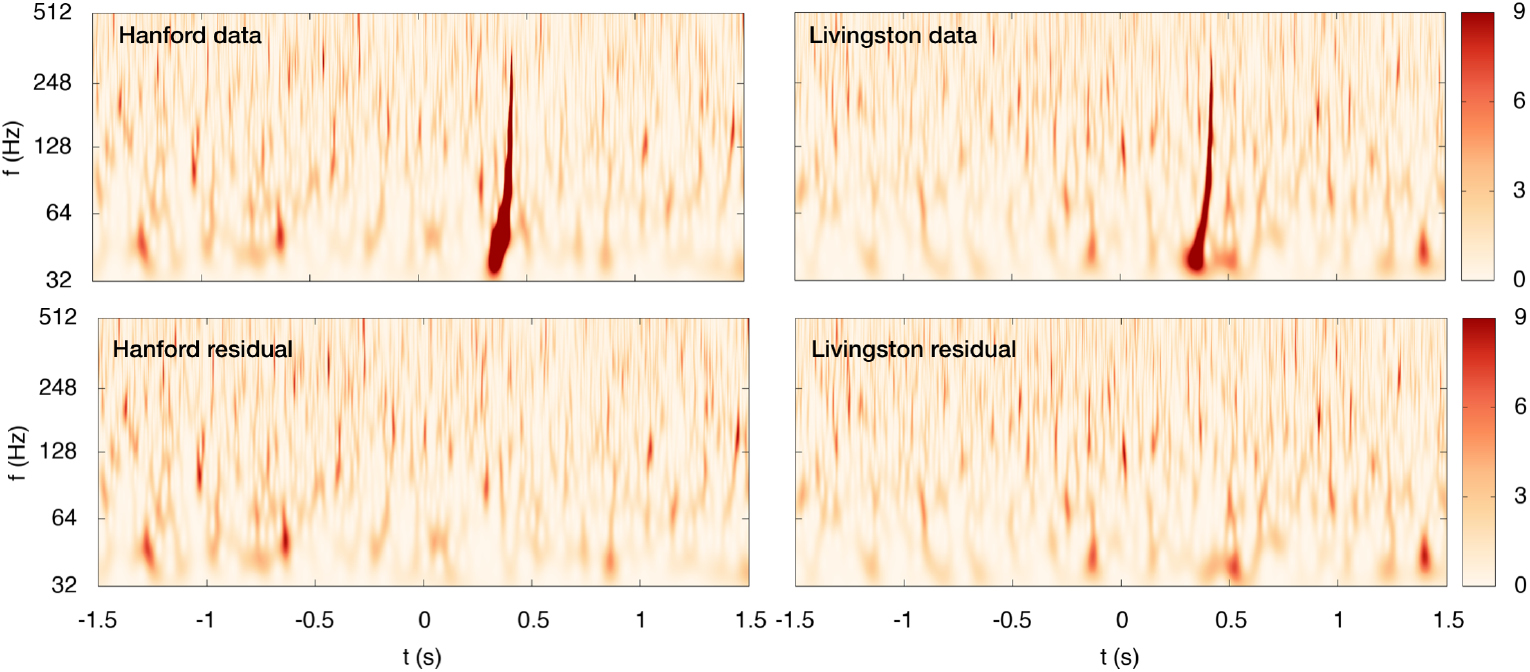
\includegraphics{img/14.jpg}
    \caption{
        LIGO-Hanford 和 LIGO-Livingston 探测器中白化数据和残差的标尺图 (或 Q 扫描) , 在围绕 GW150914事件的 $3 \t{s}$数据中. 残余物没有毛刺或相关功率. 色标, 如右侧条所示, 对应于白色的功率. 
    }
\end{figure}

除了这些定性检查外, 还可以应用更严格的定量检查. 一种常规应用的测试是使用基于小波的Bayesian 波算法[128]重新分析残差, 该算法能够识别任何毛刺和剩余的相干功率. 残差中的相干功率可能是偏离广义相对论的证据, 或者是模板模型或用于参数估计的噪声模型存在缺陷的证据. 对于任何探测到的事件, 在残差中均未发现显着的相干功率. 在GW150914的情况下, 缺乏相干残差被用来为可能偏离广义相对论[153]设定了有趣的界限. 在双中子星并合GW170817的情况下[8], 在利文斯顿探测器中, 可以看到一个巨大的非相干毛刺与信号重叠. 使用BayesWave算法重建并消除了毛刺. 一项研究显示, 毛刺消除程序是安全的, 该研究将模拟的中子星并合信号注入具有类似巨大毛刺的数据中, 然后使用BayesWave消除毛刺, 并使用LVC参数估计算法准确恢复真实信号参数[154]. 

图15显示了在去除GW150914的最大似然波形后, LIGO-Hanford和LIGO-Livingston探测器中残差的白化Fourier振幅直方图. 残差取自发现时发表的参数估计分析[127]. 这些残差被用来测试残余相干功率, 如果我们假设模板是该理论的足够准确的解, 那么可以将其描述为广义相对论的测试. 将Anderson-Darling正态性检验应用于残差, LIGO-Hanford的p值为0.15, LIGO-Livingston的p值为0.11, 表明残差与用于定义可能性的Gaussian噪声模型一致. 
\begin{figure}[htbp]
    \centering
    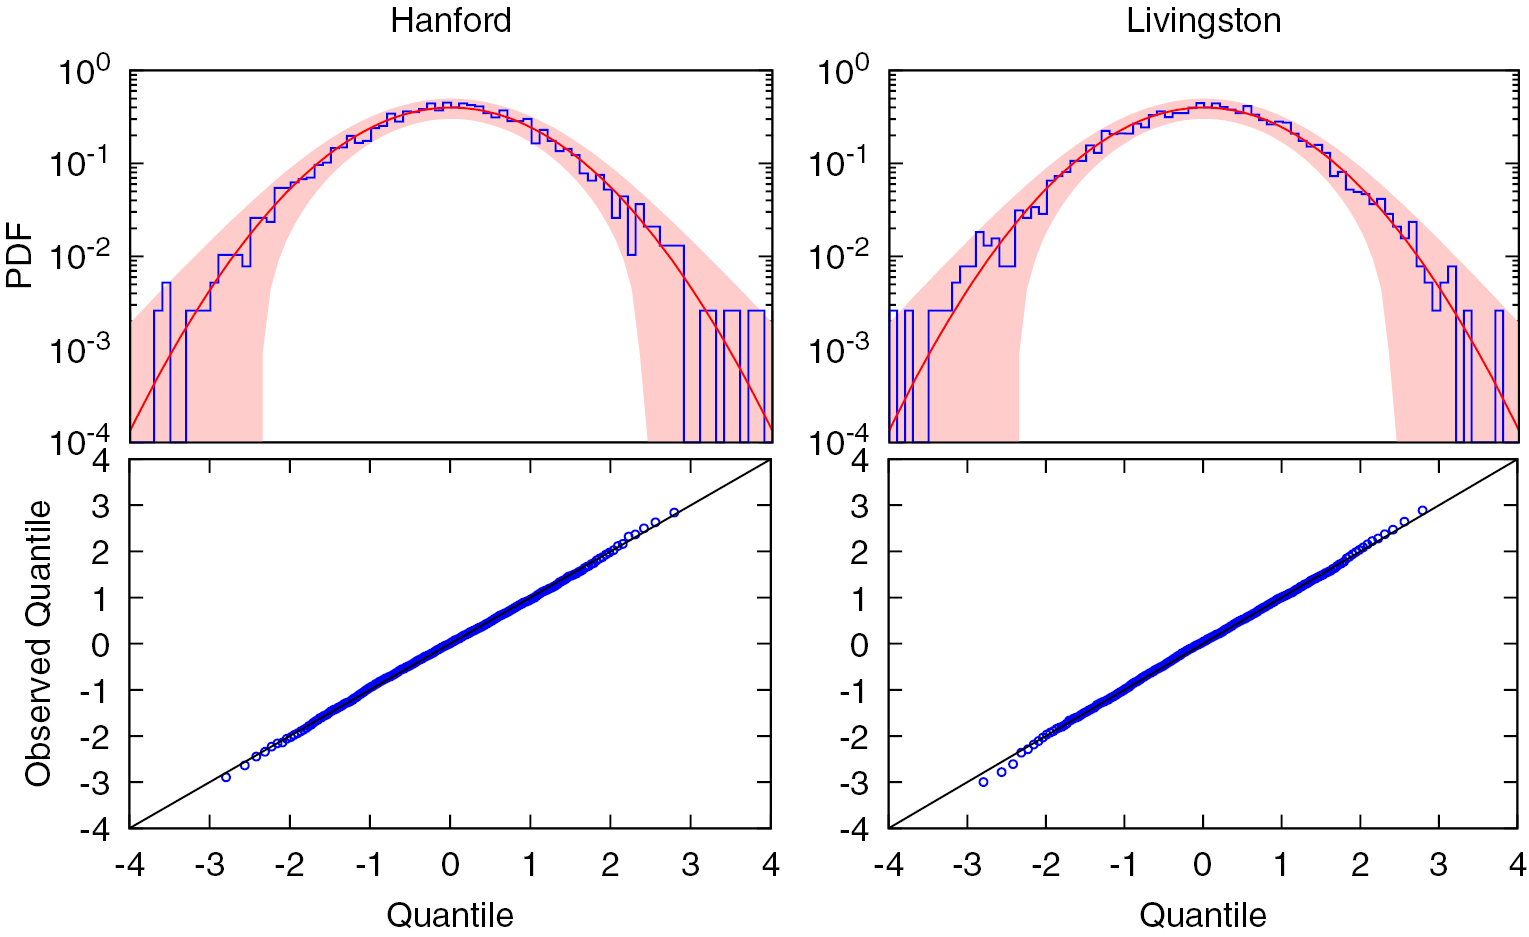
\includegraphics{img/15.jpg}
    \caption{
        LIGO-Hanford 和 LIGO-Livingston 探测器中残差的白化Fourier振幅的直方图和分位数-分位数图, 用于 $4 \t{s}$的GW150914周围数据. 上图中的阴影带表示具有有限数量的样本所导致的预期 3-$\sigma$ 方差. 残差没有显示出非Gaussian性的证据. 
    }
\end{figure}

即使残差未能通过这里讨论的稳态性和Gaussian性的形式检验, 也不一定意味着参数估计会有强烈的偏差. 当噪声偏离模型时, 分析将遭受系统性偏差. 但是, 要使这种偏差具有显着性, 与后验分布中的统计分布相比, 它必须很大. 使用模拟信号添加到真实LIGO-Virgo数据的广泛研究表明, 与统计不确定性相比, 由于噪声模型的偏差导致的系统误差通常可以忽略不计[104,143,154-157]. 一个例外是当仿真信号覆盖或重叠毛刺时间时, 在这种情况下, 偏差可能很大[158]. 当存在毛刺时, 需要使用BayesWave等工具对毛刺进行建模并消除毛刺, 理想情况下应与参数估计配合使用. 

\subsection{参数简并和可信区间}

引力波模板表现出各种参数简并, 因此具有不同参数的模板可以具有非常相似的振幅和相位演化, 并产生非常相似的可能性. 这种简并的一个例子在图13所示的GW150914组分质量的后验分布中很明显. 模板与参数之间的相似程度$\b{\lambda},  \b{\theta}$是通过匹配来衡量的
\begin{equation}
    \t{M}(\b{\lambda},\b{\theta})=\frac{(h(\b{\lambda})\mid h(\b{\theta}))}{\sqrt{(h(\b{\lambda})\mid h(\b{\lambda}))(h(\b{\theta})\mid h(\b{\theta}))}}.
\end{equation}
如果真实信号由下式描述${\b h} (\b{\lambda}) $, 则为模板的对数似然的期望值${\b h} (\b{\theta}) $, 在振幅上的最大化为
\begin{equation}
    \mathrm{E}[\ln\lambda(\b{\lambda}\mid \b{\theta})] = \frac{1}{2}\t{M}^2(\b{\lambda},\b{\theta})\t{SNR}^2,
\end{equation}
其中$\t{SNR}$是最优的信噪比[159]. 我们看到, 通过匹配测量的具有相似形态的信号会产生相似的可能性. 现在假设我们持有一个参数, $\theta^k$固定的, 然后最大化相对于所有其他参数的可能性. 直到总常数, 我们有 [159,  160]
\begin{equation}
    \ln \Lambda(\b{d}\mid\bar{\theta}^k) \equiv \max_{j=k} \ln\Lambda(\b{d}|{\theta}^j) \simeq \frac{\t{SNR}^2}{2}\t{FF}^2(\bar{\theta}^k),
\end{equation}
其中$\t{FF}^2(\bar{\theta}^k)$是波形之间的拟合因子( fitting factor)或最大匹配$\theta^k=\bar{\theta}^k$以及最大似然波形. 图 16 比较了作为GW150914的主探测器帧质量与拟合因子的最大似然值. 拟合因子作为 $m_1$ 的函数是通过最大化总体最大似然波形与具有固定 $m_1$ 的波形之间的匹配来计算的. 请注意, 此事件的后验分布具有 90\%{} 的可信区间$m_1 = 38.5_{-3.6}^{+5.6} M_\odot$, 但是, 初级质量超出此间隔的模板继续产生较大的拟合因子, 因为可以调整其他参数以部分补偿初级质量变化对波形的影响. 例如, 我们在 GW150914 的最大似然模板和主要质量为$m_1=70  M_\odot$之$\t{FF}= 0.95$.
\begin{figure}[htbp]
    \centering
    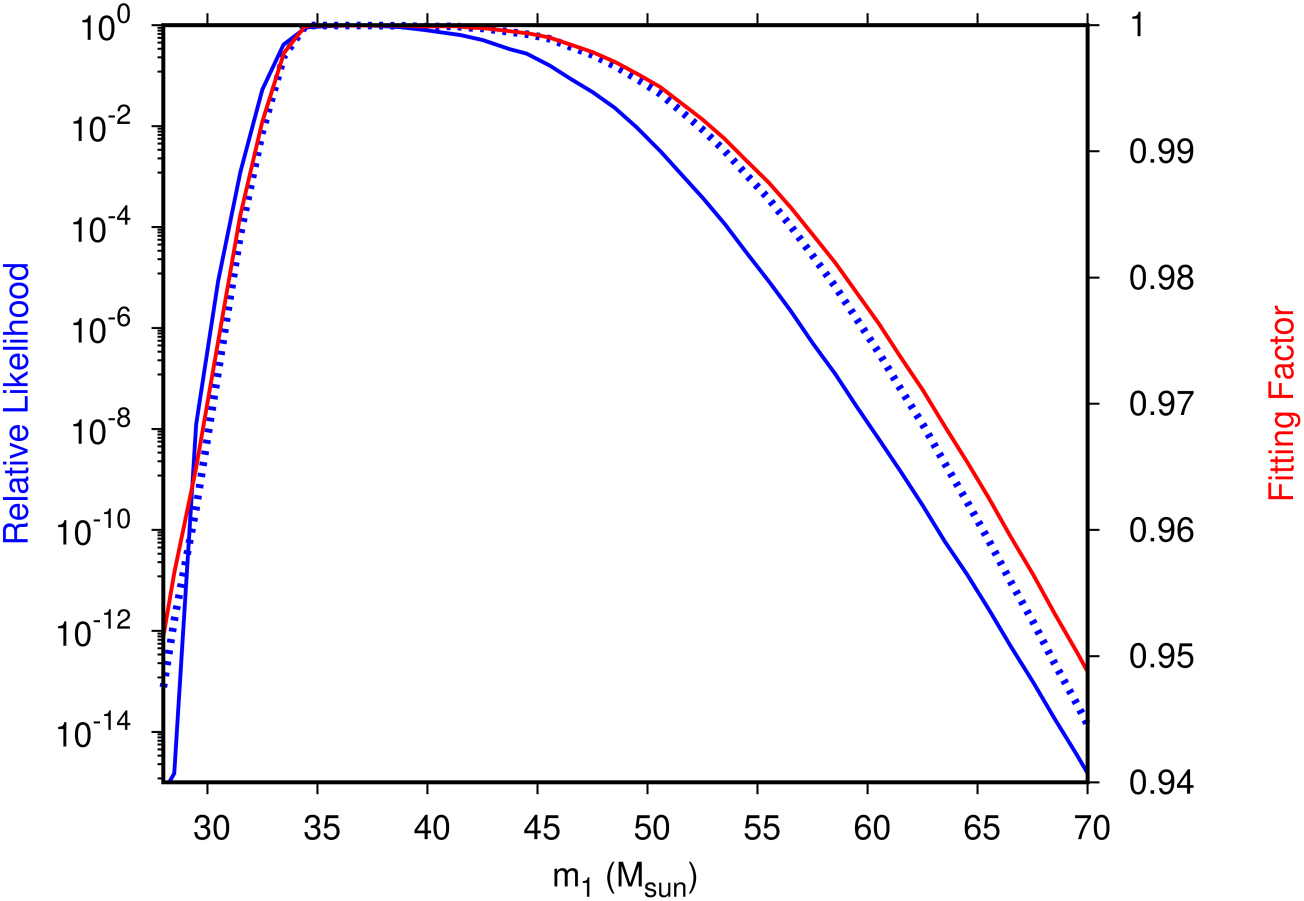
\includegraphics{img/16.jpg}
    \caption{
        似然函数 (蓝色) 和拟合因子 (红色) 作为GW150914的探测器帧初级质量 $m_1$ 的函数. 蓝色虚线表示根据公式  (31)  中的拟合因子对可能性的估计. 可能性是相对于最大似然值进行缩放的. 最大化是在次级质量, 自旋和外在参数上进行的. 
    }
\end{figure}

具有大初级质量的模板与最大似然模板之间实现高匹配或相关性的可能性已被引用为证据, 证明GW150914和其他系统的LIGO-Virgo参数估计分析可能存在缺陷[43]. 进一步假设, 由于仪器噪声不符合似然模型, 因此低估了可信区间[43]. 然而, 我们对重建的可信区域的信心来自于广泛的模拟, 这些模拟旨在比较模拟种群的累积分布与重建可信区域的累积分布. 两者之间的一致性, 参见[105]中的图10, 表明我们的算法正确地计算了可信的区间. 此外, 正如我们所展示的, GW150914的噪声属性与参数估计研究中使用的似然模型兼容, 这进一步增强了我们对用于计算可信区间的方法的信心. 

如果模板的参数在引用的可信区域之外, 则在最佳拟合模型中产生较大的拟合因子, 这并不矛盾, 因为即使是很小的模板不匹配也会对高信噪比系统 (如GW150914) 造成很大的损失. 例如, 信号与$m_1=70  M_\odot$全局最大值为$\Delta \ln {\Lambda} = -32$, 这是我们期望看到的$\t{SNR} \simeq 25$信号和拟合因子为$\t{FF}= 0.95$.但是, 较高质量解的相对可能性为$e^{\Delta \ln {\Lambda}}=10^{-13.9}$因此, 虽然具有较大初级质量的模板可以与数据产生相对良好的匹配, 但初级质量如此之高的概率微乎其微. 

\section{GW150914周围LIGO数据的残差分析}

残差的概念---数据减去模型---在引力波数据分析中起着重要作用. 如果信号模型与真实信号匹配良好, 则残差应与噪声模型$p ({\b{n}}) $, 噪声的概率分布, 的绘制一致. 在去除与独立目击者的已知相关性源后, 我们预计广泛分离的LIGO-Virgo探测器中的仪器噪声将是完全独立的, 因此每个探测器中的残差将是不相关的. 相比之下, 引力波信号将在整个探测器网络中激发相干响应, 而这种相关性的差异是我们能够将信号与噪声分离的方法之一. 

如第6节所述, 雷电可能产生相关的瞬态噪声[92], 但目前使用磁力计进行监测足以排除GW150914等事件的原因[48]. 在寻找随机引力波背景时, 低水平相关磁噪声更受关注[95-97,161].  地震噪声也受到类似的监测. 由于LIGO探测器具有相同的设计和相似的设备, 因此在随机背景和连续波引力波搜索中, 与同步时钟 (GPS) , 电力 (60 Hz) 和仪器共振相关的频率受到监测和抑制[49]. 

在本节中, 我们将使用与GW150914相关的数据来说明讨论, 但同样的考虑因素通常适用, 并且已经报告了所有重大事件的残差分析[119]. 

\subsection{信号和模板比较}

如上所述, 信号的物理参数$\b{\theta}$确定引力波信号的形状和幅度$h (t;\b{\theta}) $.数值相对论模拟可用于使用从Bayesian参数估计研究中获取的内在参数生成参考模板[24]. 然而, 仍然需要使用一组适当的外部参数将模板投影到探测器上. 在单个探测器中, 投影相当于时移, 相移和重新缩放参考模板: $\ti{ h} (\alpha,  \delta t,  \delta \phi)  (f)  = \alpha  \ti{ h}_{\t{ ref}} (f)  e^{2 \pi i f \delta t + i\delta \phi}$.

图 17 显示了 GW150914 发现论文 [1] 的图 2 中的参考数值相对论模板, 以及每个探测器的最大似然投影. 在模板的起点应用了平滑的锥度, 以避免在转换为Fourier域时出现光谱泄漏. 该模板的数据文件取自GWOSC [162]的原始发布, 源自模拟SXS:BBH:0305, 计算的系统质量比为$q = 0.819$, 自旋与轨道角动量对齐, 大小无量纲$\chi_1=0.330$和$\chi_2=-0.440$, 检测器帧总质量调整为$M=74.6 M_\odot$.这些波形参数与最终确定的波形参数一致, GW150914不确定, 但并不能完全最大化全局可能性. 使用第8节中描述的最大化程序, 可以发现信号比LIGO-Hanford探测器早$7.08\t{ms}$到达LIGO-Livingston探测器, 在LIGO-Hanford的天线响应方向图上投影的振幅为1.24倍, 相位差为-2.9弧度. 然而, 这些都是基于在固定波形下找到与探测器数据的最大似然匹配, 而不限制它们保持一致 (例如, 相对时间偏移原则上可能大于探测器之间的最大光传播时间) , 与第9节中描述的同步多探测器似然最大化相比, 这是一个简化的过程. 当数据中存在响亮的信号时, 个体和关节最大化技术会产生一致的结果. 
\begin{figure}[htbp]
    \centering
    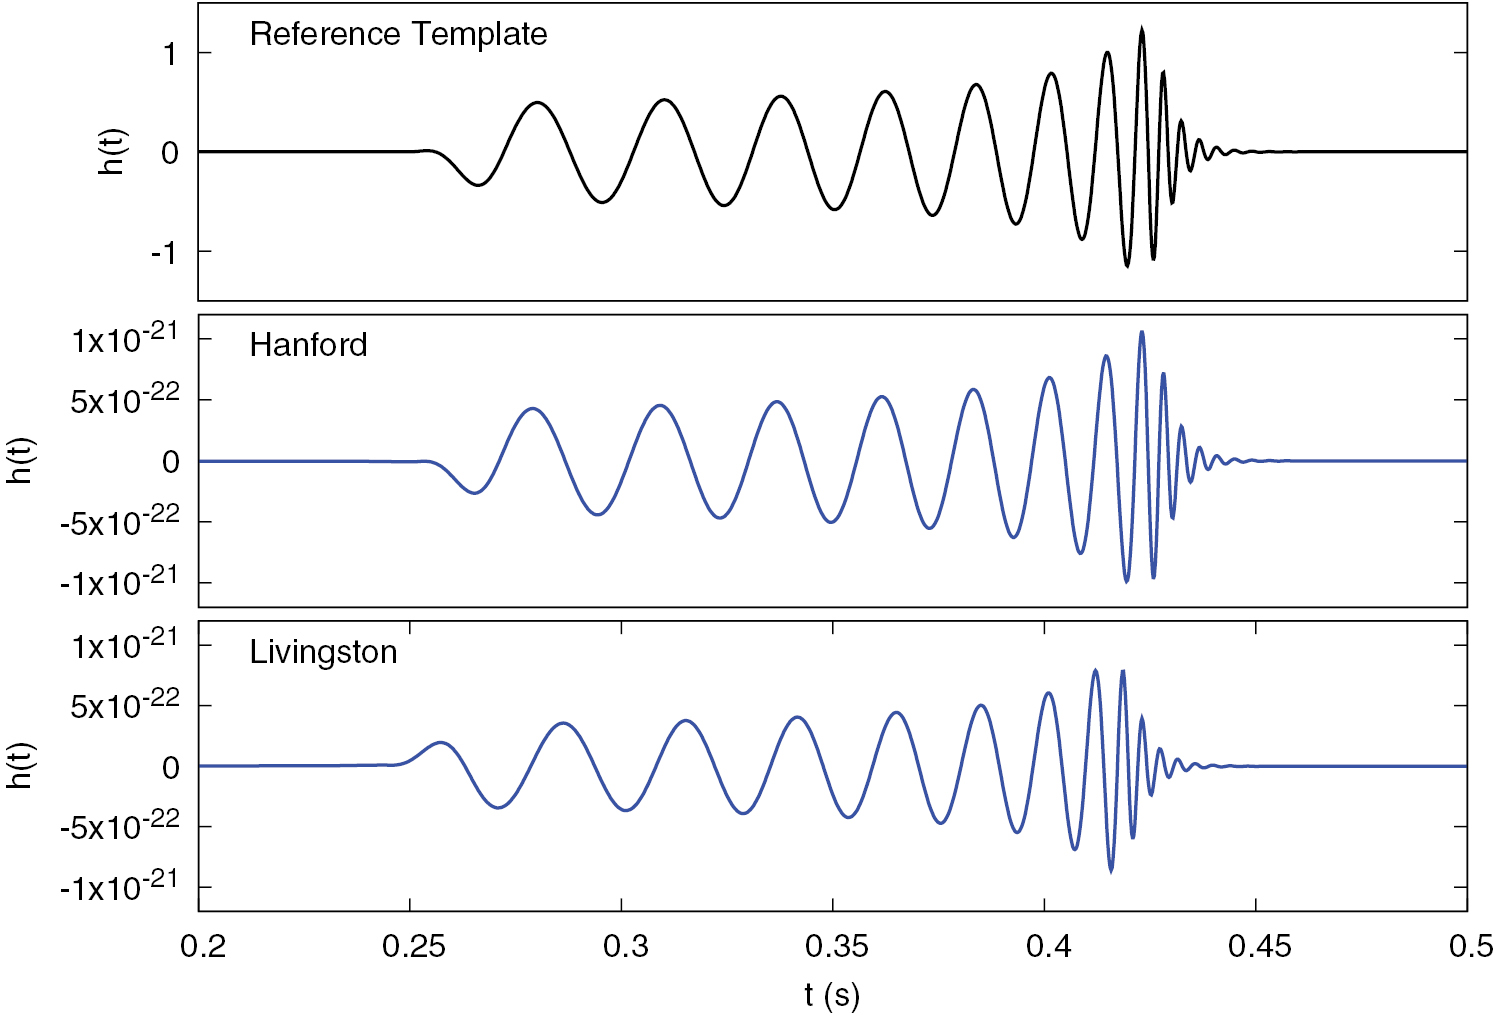
\includegraphics{img/17.jpg}
    \caption{
        GWOSC [162] 提供的用于GW150914的参考数值相对论模板如上图所示. 下方的子图显示了模板的时间, 幅度和相移版本, 这些版本分别使每个LIGO探测器的可能性最大化. 
    }
\end{figure}

在GW150914发现论文[1]的图1中, LIGO-Hanford数据被反转 (对应于相移$\pm \pi$) , 并叠加在LIGO-Livingston数据上, 以说明两个探测器中信号的相似性, 同时对原始数据进行最少的处理. 此外, 通过调整相对相位, 振幅和时间偏移, 将上述参考数值相对论模板与LIGO-Hanford和LIGO-Livingston数据近似匹配. 每个探测器的这些调整模板通过与数据相同的带通和陷波 (带阻) 滤波器, 然后减去以产生该论文中图1第三行中绘制的残差. 由于这些``PRL 图1 ''残差未进行全局优化, 而是根据滤波数据计算得出的, 因此它们产生的结果与最小化白化和带通数据中的残差的结果略有不同, 我们将在下面看到. 

图18比较了LIGO-Hanford和LIGO-Livingston探测器中白化的数据与白化数值相对论模板, 这些模板在到达时间, 振幅和相位上最大化. 此外, 还显示了从数据中减去模板所产生的残差. 在GW150914发现论文发表之前[1], 对残差进行了多次测试, 以验证它们与噪声一致. 发现每个探测器中的白化残差与Gaussian分布一致: Fourier振幅通过了Anderson-Darling检验 (参见第9节的图15) , 而发现Fourier相位是随机分布的. 使用小波重建算法[128]分析Bayesian参数估计研究[127]的残差, 该算法能够检测一般形态的相干信号. 发现GW150914残差的相干程度与噪声完全一致[153]. 
\begin{figure}[htbp]
    \centering
    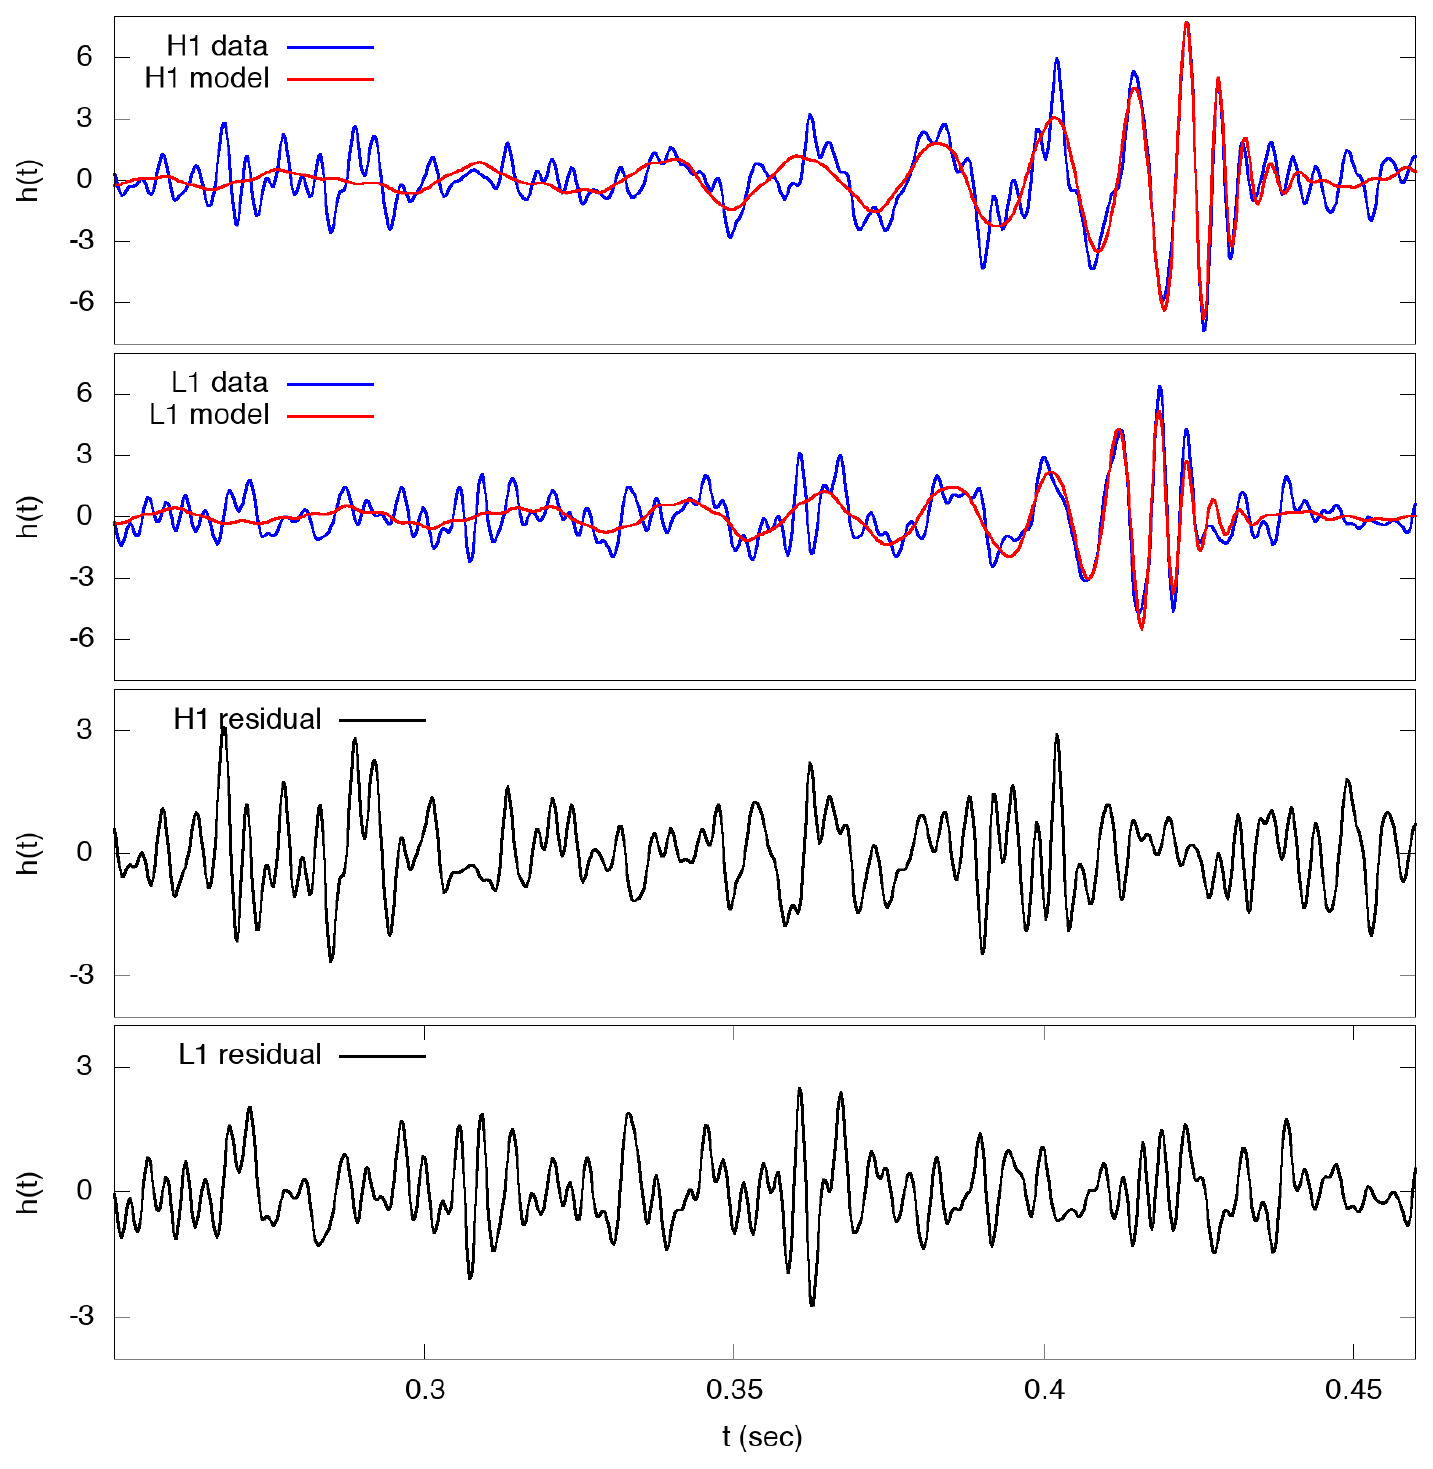
\includegraphics{img/18.jpg}
    \caption{
        上图显示了LIGO-Hanford和LIGO-Livingston探测器中相对于GPS时间1126259462的白化和带通数据. 已加白的模板叠加在数据上的最大可能性. 下方子图显示了通过从数据中减去模板而产生的残差. 
    }
\end{figure}

\subsection{相关性分析}

一种更简单但灵敏度较低的相干性测试是交叉关联两个检测器中的数据. 互相关可以在时域或频域中使用白化残差来计算. 时域中的相关性定义为: 
\begin{equation}
    C(\tau)=\frac{\int H(t-\tau)L(t)\,\d t}{\int H^2(t)\,\d t\int L^2(t)\,\d t}
\end{equation}
其中$H(t)$和$L(t)$分别表示来自LIGO-Hanford和LIGO-Livingston的数据流. 当处理持续时间为 $T$ 的有限数据段时, 数据可能会被视为周期性的: $H(t) = H (t+T) $.相关性度量对时间窗口的位置和持续时间以及应用于数据的带通滤波非常敏感. 为了对相关性的重要性做出有意义的陈述, 我们需要知道不相关白噪声的相关性度量的分布, 这些分布会根据持续时间和带通而变化. 当应用于不相关的单位方差Gaussian噪声时, 相关系数服从零均值Gaussian分布, 其方差取决于持续时间和带通. 在[42]之后, 我们将相关性分析应用于四个不同的时间窗口. Gaussian白噪声的标准差为$\sigma=0.0870$对于 $0.2 \t{s}$段, $\sigma = 0.121$对于任一$0.1 \t{s}$段和$\sigma=0.193$对于$40 \t{ms}$ 段. 

图 19 显示了使用图 18 (底部子图) 中所示的白化数据的相关性, 此外, 还显示了用于生成 GW150914 发现论文 [1] 的图 1 (顶部子图) 中用于生成子图的带通/陷波数据. LIGO-Hanford-LIGO-Livingston数据在$\sim7.3 \t{ms}$的时间滞后处存在明显的反相关峰, 这与引力波信号推断的时间延迟一致. 
\begin{figure}[htbp]
    \centering
    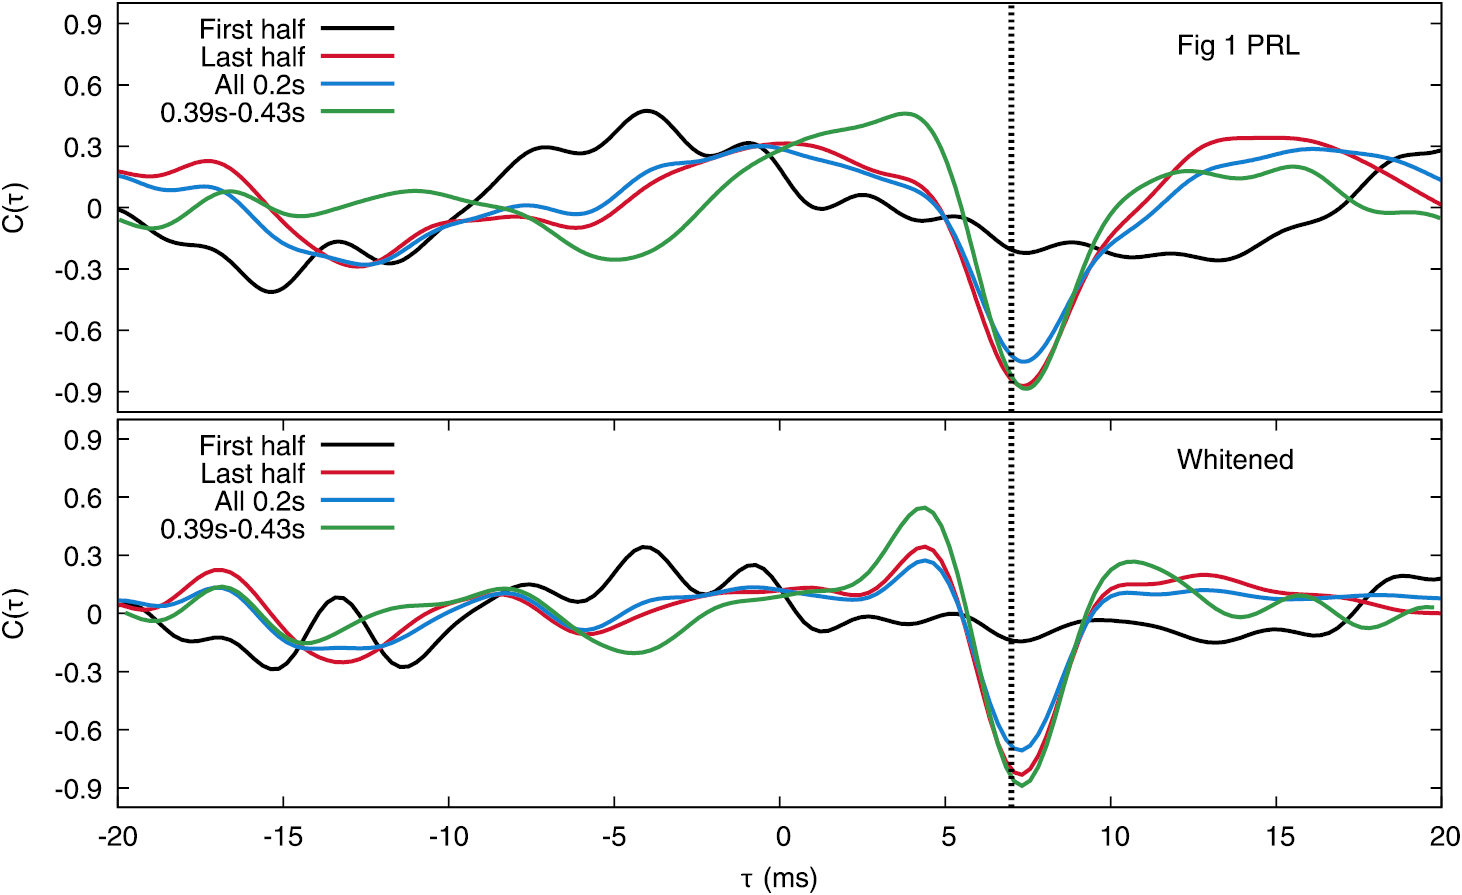
\includegraphics{img/19.jpg}
    \caption{
        LIGO-Hanford和LIGO-Livingston探测器数据之间的相关性, 使用与分析相同的四个时间间隔[42]. 一个时间间隔覆盖了图 18 中所示的全部$0.2 \t{s}$数据, 另外两个时间间隔覆盖了数据的第一个和最后$0.1 \t{s}$. 此外, 还选择了一个非常短的持续时间间隔, 持续时间为$40 \t{ms}$, 覆盖信号的峰值. $7 \t{ms}$的时间滞后将以垂直虚线的形式突出显示. 上图使用了GW150914发现论文 [1] 的图 1 中的过滤数据, 而下图则使用了图 18 中所示的白化数据. 
    }
\end{figure}

相比之下, 图 20 显示了使用上述程序产生的残差的相关性. 图18的残差在$\sim7 \t{ms}$处没有明显的反相关 (下图) , 而GW150914发现论文[1]的图1中的残差在此时间滞后处略有下降 (上图) , 反映了该论文中用于说明的参考波形不是最大似然波形. 对于最短的积分间隔, GW150914发现论文的图1中的残差在$\sim7.45 \t{ms}$的时间滞后处具有$\sim3 \sigma$反相关, 虽然与噪声略有一致, 但证明信号减法是不完美的. 相比之下, 使用幅度/时间/相位最大化的NR波形和白化数据产生的残差没有明显的偏移, 并且与噪声完全一致. 第 9 节中描述的Bayesian参数估计的残差也是如此. 对GW150914数据的独立分析也发现, Hanford和Livingston探测器中的残差之间没有显著的相关性[32,33]. 
\begin{figure}[htbp]
    \centering
    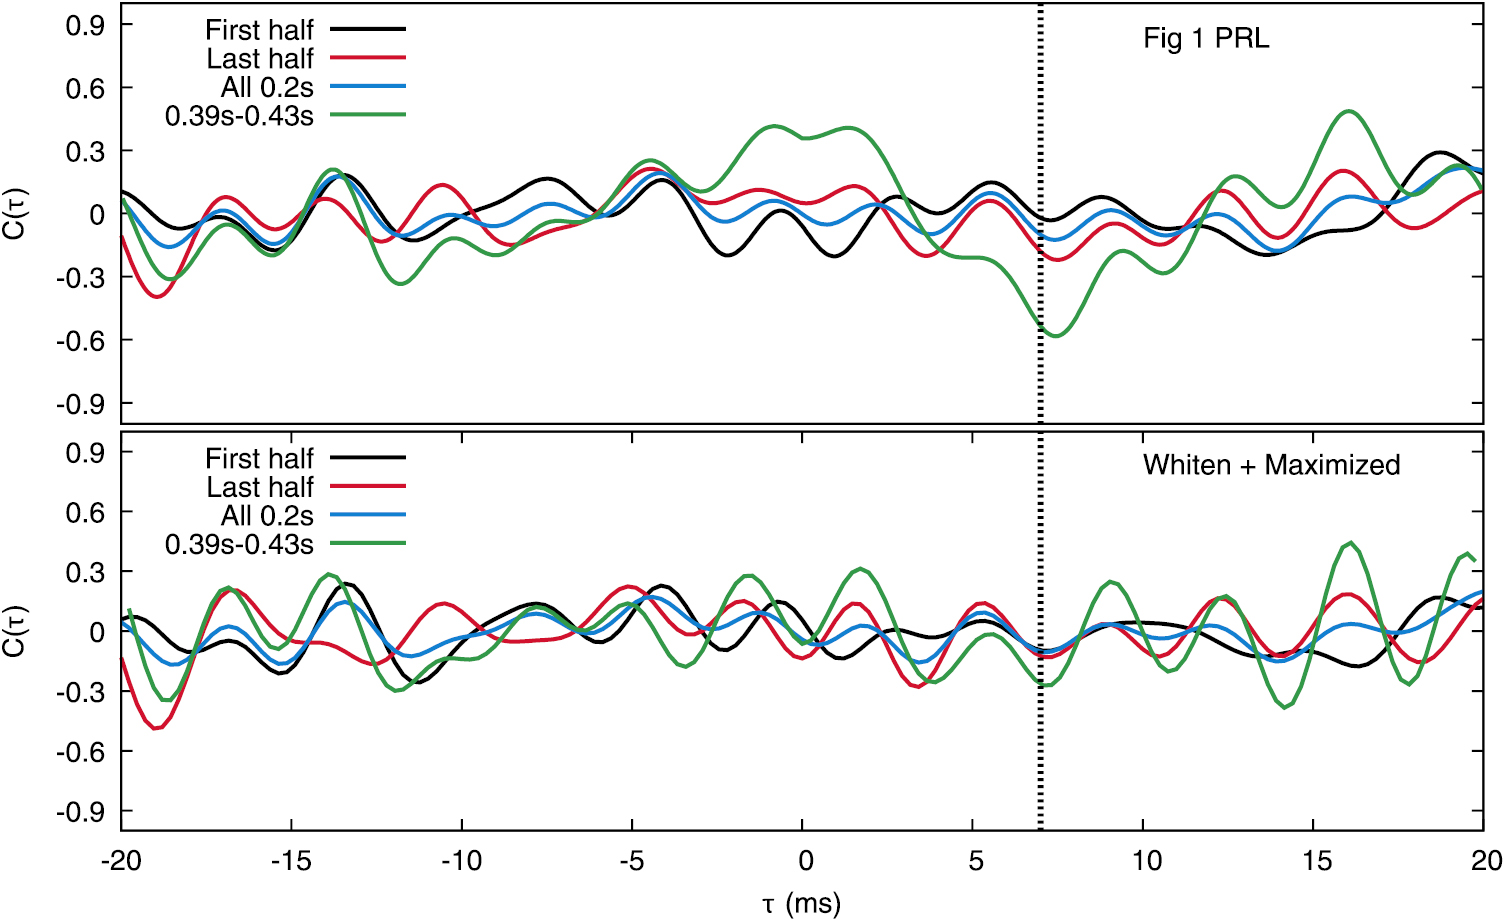
\includegraphics{img/20.jpg}
    \caption{
        LIGO-Hanford和LIGO-Livingston残差之间的相关性, 使用与图19相同的四个时间间隔. 上图使用了GW150914发现论文 [1] 的图 1 中所示的残差, 而下图则使用了图 18 中所示的白化残差时间序列. 最大似然信号减去的白化残差在任何时间窗口的任何时间滞后下都没有显着的相关性. 
    }
\end{figure}

\section{结论}

在本文中, 我们描述了LIGO和Virgo探测器的数据特性, 并概述了LVC在识别和表征来自双黑洞和双中子星系统合并的引力波信号时使用的分析方法. 我们特别仔细研究了围绕首次检测的数据, GW150914 [1,  3,  163]. 与[42]中的说法相反, 与观测到的引力波事件[119] (包括GW150914[163]) 之间没有观察到异常或意外的相关性. 独立研究人员的其他分析也对LIGO-Virgo结果的正确性得出了类似的结论[32-34,39]. 

正确处理LIGO和Virgo数据对于正确进行分析至关重要. 例如, 在本文中, 我们使用了白化的最大似然波形 (如第9节和第10节所述) 作为GW150914, 当从数据中减去时, 产生的残差与Gaussian噪声一致, 并且不同检波器之间没有相关性. 如果从数据中减去的模板波形与真实的引力波信号不够匹配, 那么该信号的其余部分将在产生的残差中存活, 因此可能表现出非平凡的相关性. 

[1]的图1的构造是为了尽可能简单地显示信号与广义相对论兼容. 它没有说明完整的LSC-Virgo统计数据分析. 该图在[1]中被描述为LIGO探测器上引力波信号的可视化, 并与一种与引力波数据一致的数值相对论波形的比较. 关于数值相对论波形和[1]的图1的残差的统计声明并不打算, 尽管不幸的是, 该图可能是以这种方式解释的. 

LVC对GW150914信号和周围噪声进行了广泛的统计研究, 这些研究记录在[127]中. 请注意, 在用于发现的参数估计配套论文中提出了GW150914的白化时间序列;参见[127]的图6. 这些研究, 以及这里给出的更简单的研究, 都支持了这样一种解释, 即信号与广义相对论的黑洞合并解非常匹配. 这一结论的有效性得到了LVC后续数据和分析的支持 (包括对观测运行O1和O2中检测到的所有双黑洞产生的引力波信号的研究[119]) 以及独立分析. 

Advanced LIGO和Advanced Virgo的引力波数据可以被描述为局部稳态和Gaussian, 当存在毛刺时会出现偏差. LVC进行了大量的数据质量, 检测器表征和校准研究, 以便对报告的检测结果充满信心[47,48,50,74]. 

然而, 没有必要假设数据是稳态的和Gaussian的, 以高置信度搜索和检测来自紧双星聚结的引力波. 取而代之的是, LIGO-Virgo对引力波的搜索使用各种方法来直接从数据中估计假警报率, 例如, 通过在探测器之间引入相对时间偏移. 

先前的研究还表明, LVC的参数估计结果是可靠的[104,143,154-157]. 对于来自双中子星合并的引力波, 参数估计程序也很稳健, GW170817 LIGO-Livingston数据中存在噪声毛刺, 与引力波信号重叠[8,154]. LVC以外的研究人员获得的GW170817参数估计值与LVC分析相当, 并支持LVC分析的结论[3537];这些研究是通过公开发布引力波数据来实现的[24]. 

虽然本文中的例子集中在GW150914和GW170817的事件上, 但所提出的结论已被证明对于分析包含LIGO和Virgo迄今为止探测到的所有11个引力波事件的数据是有效的[3,119]. 随着LIGO和Virgo的合作报告了更多的事件[3,164], 更广泛的科学界对与这些事件相关的数据进行独立分析将非常有价值, 并可能产生新的见解. 为此, 本文试图就LIGO和Virgo探测器噪声的性质以及引力波信号的提取提供一些指导. LVC鼓励科学界分析其数据;LIGO和Virgo的数据将继续在GWOSC网站上公开提供[24]. 

\end{document}
